\documentclass[conference]{IEEEtran}
\usepackage{amsmath,amssymb,amsthm}
\usepackage{stmaryrd}
\usepackage{booktabs,array,multirow,tabularx,threeparttable}
\usepackage{xcolor}
\usepackage{tikz}
\usetikzlibrary{arrows.meta,positioning,shapes.geometric,fit,backgrounds,calc}
\usepackage{pgfplots}
\pgfplotsset{compat=1.17}
\usepackage{algorithm}
\usepackage{algpseudocode}
\usepackage{enumitem}
\usepackage{cite}
\usepackage{url}
\usepackage{microtype}

\definecolor{accent}{HTML}{0B5394}
\definecolor{accentlight}{HTML}{D9E8F7}
\definecolor{warn}{HTML}{B45F06}
\definecolor{okgreen}{HTML}{38761D}
\definecolor{ledger}{HTML}{674EA7}

\newtheorem{definition}{Definition}
\newtheorem{proposition}{Proposition}
\newtheorem{corollary}{Corollary}
\newtheorem{remark}{Remark}
\newtheorem{assumption}{Assumption}
\newtheorem{theorem}{Theorem}

\newcommand{\Ione}{\ensuremath{I_1}}
\newcommand{\Itwo}{\ensuremath{I_2}}
\newcommand{\Ithree}{\ensuremath{I_3}}
\newcommand{\Ifour}{\ensuremath{I_4}}
\providecommand{\tc}{\tau_{c}}
\providecommand{\meet}{\sqcap}
\providecommand{\DeltaIrrel}{\Delta_{\mathrm{irrel}}}
\providecommand{\Dirr}{D_{\mathrm{irr}}}
\providecommand{\Lift}{\mathrm{Lift}}
\providecommand{\Tr}{\Sigma}
\newcommand{\att}{\ensuremath{\mathsf{att}}}
\newcommand{\cert}{\ensuremath{\mathsf{cert}}}
\newcommand{\deps}{\ensuremath{\mathsf{dep}}}
\newcommand{\support}{\ensuremath{\mathsf{support}}}
\newcommand{\acts}{\ensuremath{\mathsf{acts}}}
\newcommand{\ev}[1]{\ensuremath{\mathsf{#1}}}
\newcommand{\lmin}{\ensuremath{\ell_{\min}}}
\newcommand{\lreq}{\ensuremath{\ell_{\mathrm{req}}}}
\newcommand{\Cprot}{\ensuremath{C_{\mathrm{prot}}}}
\newcommand{\Dirrel}{\ensuremath{\Delta_{\mathrm{irrel}}}}
\newcommand{\dist}{\ensuremath{\mathsf{dist}}}
\newcommand{\DEI}{\ensuremath{\mathrm{DEI}}}
% ==== GATE MEASURED VALUES (results_gate/*.json, 2026-08-02; offline cache replay) ====
\newcommand{\GateFollows}{4}
\newcommand{\GateQuar}{2}
\newcommand{\GateHonestUnch}{1}
\newcommand{\GateInterUnch}{1}
\newcommand{\GateBenignDestr}{3}
\newcommand{\GateFalseQuarN}{0}
\newcommand{\GateFalseQuar}{0\%}
\newcommand{\GateOverhead}{1.375}
\newcommand{\GateMonitorUs}{52}
\newcommand{\tick}{\ensuremath{\checkmark}}
\newcommand{\partl}{\ensuremath{\sim}}
\newcommand{\absent}{---}

% ===== NON-ANONYMIZED AUTHOR METADATA (for camera-ready; submission stays anonymous) =====
% [author line removed; author metadata is kept outside the Overleaf project until camera-ready]
% [author line removed; author metadata is kept outside the Overleaf project until camera-ready]
% [author line removed; author metadata is kept outside the Overleaf project until camera-ready]
% ============================================================================

\begin{document}
\input{results_macros}  % auto-generated live-model numbers (swap n by rerunning recompute)


\title{Epistemic Security: A Formal, Falsifiable\\ Definition of
Decision-Level Epistemic Integrity for Agentic AI}

\author{\IEEEauthorblockN{Anonymous Author(s)}
\IEEEauthorblockA{NDSS 2027 Submission}}

\IEEEoverridecommandlockouts
\makeatletter\def\@IEEEpubidpullup{6.5\baselineskip}\makeatother
\IEEEpubid{\parbox{\columnwidth}{
		Network and Distributed System Security (NDSS) Symposium 2027\\
		22--26 March 2027, Seoul, Republic of Korea\\
		ISBN 978-1-970672-09-1\\
		https://dx.doi.org/10.14722/ndss.2027.24xxxx\\
		www.ndss-symposium.org
}
\hspace{\columnsep}\makebox[\columnwidth]{}}

\maketitle

\begin{abstract}
Agentic AI systems deployed over the Model Context Protocol (MCP)
act on beliefs assembled from content their adversaries can write:
retrieved documents, tool results, and persistent memory. Deployed
defenses constrain what such systems may \emph{do}; none states
formally what it means for their \emph{conclusions} to be
trustworthy, nor which part a runtime monitor can enforce. We
define \emph{decision-level epistemic integrity} (DEI) over
decision traces as four invariants: provenance-completeness,
integrity non-degradation, evidential-support sufficiency, and a
counterfactual-dependence bound. We prove the first three are
safety properties enforceable by execution monitoring; the fourth
is a 2-safety hyperproperty no single-trace monitor can check, and
each invariant carries a refutation condition. We instantiate the
enforceable fragment in CZTA, a zero-trust MCP gateway (0.20\,ms
p50 overhead), and evaluate it on AgentDojo with a real model.
Enforcement blocks 10.3\% of authorized actions. The predicted
rationalization attack, an injection-chosen action laundered under
attested support, executes end-to-end and reproduces a coverage
counterexample the auditable fragment detects. A counterfactual
audit gate then re-commits irreversible actions under
pre-registered perturbations and quarantines both laundering
admissions at \GateFalseQuar{} false-quarantine. On a live
frontier model (gemini-2.5-flash), where the canonical AgentDojo
injection succeeds in 45\% of episodes (18/40), the enforceable
fragment reduces attack success to 5\% (2/40), an 89\% relative
reduction (Fisher exact $p<10^{-4}$), at a utility cost that
$n{=}24$ per arm cannot distinguish from the no-defense baseline
(70.8\% vs.\ 83.3\% benign completion, Fisher $p{=}0.49$). An
open-weight family shows no susceptibility to the same attack,
evidence that susceptibility is model-specific and benchmark
obsolescence premature. DEI is grounded in a
registered PRISMA-ScR review (552 core records) with a hash-sealed
reliability audit ($n=114$) mapping each attack class to the
invariant it violates.
\end{abstract}

\begin{IEEEkeywords}
agentic AI security, epistemic integrity, runtime verification,
reference monitors, zero trust, Model Context Protocol, prompt
injection
\end{IEEEkeywords}

\section{Introduction}
An agentic AI system is an epistemic machine before it is an
acting one: it reads, retrieves, remembers, and only then invokes
tools with real-world effects. Its adversaries have noticed.
Indirect prompt injection, tool and Model Context Protocol (MCP)
poisoning, retrieval and memory poisoning, and curated context all
attack the same surface: not the action interface but the
\emph{evidential basis} on which actions are chosen. Defenses have
answered at the action interface: information-flow and capability
designs~\cite{camel}, execution-boundary authority checks~\cite{cxi},
guardrail agents~\cite{guardagent}, and influence tracking~\cite{argus}
constrain what a compromised agent may do. What none of them states
is the property they are all reaching for: what it means for an
agent's conclusions to be trustworthy, and which parts of that
property anyone can actually enforce at runtime.

This paper supplies that missing object. We define
\emph{decision-level epistemic integrity} (DEI) formally, over
decision traces of evidence, provenance, belief state, and action,
as four invariants: provenance-completeness, integrity
non-degradation, evidential-support sufficiency, and a
counterfactual-dependence bound (\S\ref{sec:definition}). The
definition is built to be honest about enforcement: we prove the
first three invariants are safety properties (runtime-monitorable
and, more strongly, enforceable by execution monitoring in
Schneider's classical sense) while the fourth is a 2-safety
hyperproperty that provably cannot be checked by any monitor
observing a single trace (\S\ref{sec:monitorability}). It is also
built to be refutable: each invariant carries a stated falsifying
observation, and the definition as a whole is falsified by any
successful attack on an invariant-satisfying execution
(\S\ref{sec:falsifiability}).

The term needs one disambiguation. Concurrent work uses ``epistemic
integrity'' for an architectural reliability property of
long-running agents~\cite{shen}, and an older literature for
societal information-ecosystem resilience~\cite{seger}; DEI is a
falsifiable security property of single decisions, stated against
an attacker model and classified by what a runtime monitor can
enforce.

This is a systems paper with a formal spine, not the reverse.
Every definition in \S\ref{sec:definition} exists to be checked by
a gateway in front of a live MCP deployment, and every proposition
ends in a measurement: the safety invariants cost a measured
authorization overhead (Table~\ref{tab:overhead}) to enforce in
CZTA, our zero-trust reference monitor (\S\ref{sec:czta}), and the
auditable invariant is exercised against a real model on an
AgentDojo-scale workload, where we measure the operating point
under enforcement and execute the rationalization attack the
definition predicts (\S\ref{sec:workload}); the authorization
layer is checked separately at the composition boundary
(\S\ref{sec:redteam}). We score the campaign not as a demo but as
a test of the theory's coverage claim.

The definition does not float free of the threat landscape it
formalizes. It is grounded in a PRISMA-ScR scoping review of the
epistemic attack surface with a registered human-reliability audit
(\S\ref{sec:review}), and the review's attack taxonomy is mapped
class-by-class onto the invariants each attack must violate
(\S\ref{sec:crosswalk}): pre-registered predictions the red team
then tests.

\paragraph*{Contributions}
\begin{itemize}[leftmargin=1.15em,itemsep=1pt]
\item \textbf{A formal, falsifiable definition} of decision-level
epistemic integrity (\S\ref{sec:definition}): four invariants over
decision traces, stated relative to an explicit, minimized
epistemic TCB, each carrying a refutation condition.
\item \textbf{An enforceable/auditable separation with proof}
(\S\ref{sec:monitorability}): the contribution is the
decomposition, not the classical machinery: DEI factors into
exactly three invariants (\Ione--\Ithree) enforceable by execution
monitoring plus one (\Ifour) that is a 2-safety hyperproperty
provably not enforceable by any single-trace monitor. That the
boundary falls where it does, and is principled rather than
definitional, is the result, drawn by classical theorems, not by
hope.
\item \textbf{A falsifiability protocol}
(\S\ref{sec:falsifiability}): per-invariant refutation conditions
plus a coverage criterion under which a successful attack on an
invariant-satisfying execution falsifies the definition
itself, turning red-teaming into a test of the theory and
answering the call for adaptive evaluation of action-level
defenses~\cite{oob}.
\item \textbf{CZTA, an existence proof} (\S\ref{sec:czta}): a
zero-trust gateway over a live MCP deployment instantiating the
enforceable invariants, with measured authorization overhead and
per-pattern red-team results scored against the coverage claim,
including the detected-not-prevented result of \S\ref{sec:rugpull}. CZTA
demonstrates feasibility; it is not itself claimed as a
contribution.
\item \textbf{A workload-scale and live-model evaluation}
(\S\ref{sec:workload}, \S\ref{sec:livemodel}): on the AgentDojo workspace suite we
instantiate the policy objects concretely, measure the
security/utility operating point under enforcement (10.3\%
false-block on user-authorized actions; Wilson 95\,\%
$[3.6, 26.4]$), and \emph{execute} the
rationalization attack, reproducing end-to-end the coverage
counterexample the enforceable fragment cannot prevent and the
auditable fragment detects, reported per the falsification
protocol. On a live frontier model that follows the canonical
injection $45\%$ of the time, the enforceable fragment reduces
attack success to $5\%$ ($89\%$ relative reduction, $p<10^{-4}$) at a
utility cost not statistically resolvable at $n{=}24$ per arm
($p{=}0.49$), while an open-weight family shows no susceptibility to
the same attack---evidence that
susceptibility is model-specific and that benchmark obsolescence
is premature.
\item \textbf{A counterfactual audit gate for irreversible actions}
(\S\ref{sec:gate}): the auditable invariant deployed as a bounded,
decision-local pre-execution check (quarantining \GateQuar{} of
\GateFollows{} laundering follows at \GateFalseQuar{}
false-quarantine and \GateOverhead$\times$ benign model-time
overhead), converting the coverage counterexample into a
countermeasure with measured cost.
\item \textbf{An audited map of the epistemic attack surface}
(\S\ref{sec:review}): a PRISMA-ScR scoping review with a
registered human-reliability audit ($n=114$ frozen sample), and a
class-by-class crosswalk from the attack taxonomy to the
invariants (\S\ref{sec:crosswalk}).
\end{itemize}

\paragraph*{Scope of the novelty claim}
Within the scope of our registered search and its update (arXiv
cs.CR/cs.AI/cs.CL/cs.SE and the major security venues, through
17~July~2026; \S\ref{sec:delta}), no prior work provides a formal,
falsifiable definition of decision-level epistemic integrity that
separates runtime-enforceable from auditable-only invariants with
supporting theory and instantiates the enforceable fragment in a
working monitor (Table~\ref{tab:positioning}). The closest prior formalization states judgment
integrity as an invariance condition without a monitor or
monitorability analysis~\cite{qu}; the closest prior use of the
term characterizes an architecture qualitatively~\cite{shen}. We
claim neither first use of the phrase nor first statement of
decision invariance.

\section{Related Work}
\label{sec:related}

\subsection{Pre-Freeze Landscape (Registered Search Through May 2026)}

\paragraph{In-band defenses and their failure mode}
Indirect prompt injection (adversarial instructions planted in
content an agent will retrieve) was identified early as the
structural risk of tool-using LLM systems~\cite{greshake}. A first
generation of defenses operated in band: detection classifiers,
prompt hygiene, and instruction-hierarchy fine-tuning. Adaptive
evaluations have repeatedly broken such defenses, motivating the
position that in-band immunity may be unattainable in
principle~\cite{abdelnabi} and pushing the field toward
system-level enforcement.

\paragraph{Out-of-band enforcement: the CaMeL lineage}
CaMeL interposes a protective layer that separates control flow
from data flow and attaches capability metadata to values,
securing a majority of AgentDojo tasks by design rather than by
model robustness~\cite{camel}. A family of successors (FIDES,
Progent, RTBAS, Conseca, FORGE, and related systems, systematized
in~\cite{oob}) varies the mechanism (information-flow labels,
policy languages, taint propagation) but shares the architecture:
a deterministic reference monitor outside the model. Guardrail
agents such as GuardAgent take a complementary route, compiling
natural-language guard requests into executable checks over
another agent's actions~\cite{guardagent}. Zero-trust MCP gateway prototypes bind caller identity and
capability policy off-host~\cite{ztmcp,kodathala2026aiauthz}:
they decide who may call what, not what may count as a reason for
the call. Our work supplies what
this line has lacked: a formal statement of the decision-level
property these monitors approximate, with a proof-backed boundary
between what they can enforce and what they can only audit.

\paragraph{Benchmarks}
AgentDojo established the live-environment evaluation standard for
injection attacks on tool-using agents~\cite{agentdojo}; successor
and sibling suites (InjecAgent, Agent Security Bench, MCP-specific
benchmarks, and memory/RAG-poisoning suites) are consolidated,
with consistency caveats, in~\cite{benchtax}. We use these to
situate our red-team campaign's scope, not as its substrate: our
campaign attacks a live MCP deployment (\S\ref{sec:czta}).

\paragraph{MCP and protocol-surface security}
The Model Context Protocol standardized tool connectivity and, in
its current revision, authorization for remote
servers~\cite{mcpspec}; community taxonomies rank tool poisoning
among its principal risks and analyze where in the stack defenses
can be placed~\cite{owaspmcp,mcpdpt}. These secure the transport
and authorization surface CZTA sits on; none addresses what the
agent may \emph{conclude} from what it reads.

\paragraph{Classical foundations}
\DEI{} deliberately builds on machinery with decades of
scrutiny---integrity lattices, well-formed transactions,
noninterference, decentralized IFC, provenance semantics, evidence
theory, and the runtime-verification canon---applied to a new
object (the epistemic state of an agentic system), not a new
logic; App.~\ref{app:foundations} gives the full lineage with
citations.

\paragraph{Out-of-band defenses and their evaluation}
A systematization of out-of-band defenses casts CaMeL, FIDES,
Progent, and successors as instances of Biba integrity, reference
monitoring, and least privilege, and identifies two open problems:
these defenses have been validated almost exclusively on static
benchmarks, and their trusted base (provenance assignment) is
under-specified~\cite{oob}. Both observations shape
\S\ref{sec:definition}: we name and minimize the epistemic TCB
explicitly, and our falsifiability protocol is an adaptive
evaluation design in which an attacker must either trip a
monitored invariant or produce a coverage counterexample. Related
runtime systems have converged on influence- and
provenance-tracking: ARGUS builds an influence provenance graph
and verifies that decisions are justified by trustworthy evidence
before execution~\cite{argus}; provenance/authorization dual-graph
designs and execution-provenance surveys chart the same
territory~\cite{tracessurvey}. These systems are the natural
instantiation peers of CZTA; none states the property they
approximate as a formal definition, which is the
division of labor we propose. The Biba discipline is also machine-checked for agent memory
stores~\cite{louck2026tmanm}; CZTA applies it to the decision's
evidential basis at action time rather than to the store. Complementing the defenses,
principled skepticism about in-band robustness~\cite{abdelnabi}
and consolidated benchmark taxonomies~\cite{benchtax} sharpen why
the enforceable/auditable boundary must be drawn honestly rather
than promised away.

\paragraph{Deployment posture}
Frontier-lab guidance now treats internal agents as potentially
compromised insiders and adopts zero trust for agent
infrastructure~\cite{controlroadmap}, converging on the threat
model of \S\ref{sec:threat}. On the protocol surface, MCP
hardening has matured (authorization in the current spec; attack
taxonomies and defense-placement analyses~\cite{mcpspec,owaspmcp,mcpdpt}),
situating CZTA's gateway placement but not addressing the decision
layer.

\paragraph{Terminological note}
``Epistemic security'' also names a societal research program on
protecting information ecosystems~\cite{seger}; we use the term in
a narrower technical sense---the integrity of a single agent
system's evidential basis for consequential actions.

\subsection{Search Refreeze and the 2026 Delta}
\label{sec:delta}
Our registered literature search was frozen in May 2026; because
the field moved materially in the following ten weeks, we executed
a registered search update (identical queries and sources,
date-restricted 1~May--17~July~2026) and report the delta here
rather than silently absorbing it. Three developments matter for
this paper's claims.

\paragraph{Integrity framings for agents}
Qu et al.\ argue that securing LLM agents requires
intent-to-execution integrity (the conjunction of tool,
instruction, judgment, and data-flow integrity) and give
\emph{judgment integrity} an invariance form: task-irrelevant
perturbations of untrusted data must not change the
decision~\cite{qu}. This is the closest prior formalization to our
\Ifour, and we adopt its invariance condition; the position paper
itself notes that judgment integrity is the hardest of the four to
formalize and stops short of a monitor, a monitorability analysis,
or a falsification protocol: the gap \S\ref{sec:definition}
fills. Independently, Shen introduces \emph{agent epistemic
integrity} as a first-class architectural constraint for
long-running agents: belief, capability, and goal commitments must
remain meaningful across independently evolving model and harness
layers, secured by an explicit model--harness interface
contract~\cite{shen}. We share the diagnosis but differ in kind:
that work prescribes an architecture and a contract hierarchy,
whereas we give a formal definition over decision traces with
enforceable and auditable fragments distinguished by proof. At the
execution boundary, context-to-execution integrity (CXI) requires
protected sink fields, sink-interpreted effects, and invocation
events to carry authority binding to the same action manifest
before a proposal becomes executable, with a deterministic
admission gate evaluated on AgentDojo-scale corpora (720 live
episodes; a 400-episode code-agent benchmark with zero observed
escapes)~\cite{cxi}; CXI secures the sink layer and explicitly
disclaims model-level noninterference; it composes beneath our
decision layer rather than competing with it.

\begin{table}[t]
\centering
\caption{Positioning against the closest prior work.
$\tick$ = provided; $\partl$ = partial; --- = absent.
\emph{Split} = runtime-enforceable separated from auditable-only
guarantees, with supporting theory. All rows verified against the
public record on 17 July 2026.}
\label{tab:positioning}
\scriptsize
\setlength{\tabcolsep}{3pt}
\begin{tabularx}{\columnwidth}{@{}>{\raggedright\arraybackslash}X c c c c c >{\centering\arraybackslash}p{1.05cm}@{}}
\toprule
& Def. & Falsif. & Monit. & Split & Runtime & Dec.-layer \\
\midrule
CaMeL~\cite{camel} & \absent & \absent & \absent & \absent & \tick & \absent \\
GuardAgent~\cite{guardagent} & \absent & \absent & \absent & \absent & \tick & \partl \\
Intent-to-exec.~\cite{qu} & \partl & \absent & \absent & \absent & \absent & \tick \\
Agent epist.\ int.~\cite{shen} & \partl & \absent & \absent & \absent & \absent & \tick \\
CXI~\cite{cxi} & \tick & \absent & \absent & \partl & \tick & \absent \\
ARGUS~\cite{argus} & \absent & \absent & \absent & \absent & \tick & \partl \\
OOB systematization~\cite{oob} & \absent & \partl & \absent & \absent & \absent & \partl \\
\midrule
\textbf{This work} & \tick & \tick & \tick & \tick & \tick\,(exist.\ proof) & \tick \\
\bottomrule
\end{tabularx}
\end{table}

\section{The Epistemic Attack Surface: Scoping Review and
Reliability Audit}
\label{sec:review}

\subsection{Review Protocol and Corpus}
We conducted a PRISMA-ScR scoping review~\cite{prisma} of attacks
and defenses on the epistemic layer of agentic AI systems under a
registered protocol. Automated screening across six databases,
each queried with three strategies crossing an agentic-AI
population facet with an epistemic-attack facet, restricted to
2017--2026 with backward snowballing (per-database strings and
executed counts in Appendix~\ref{app:search}, Table~\ref{tab:search}),
identified 6{,}512 records; after removing 4{,}129 duplicates,
2{,}383 unique records were screened at title/abstract, of which
552 were retained as the core evidence tier and 931 as a
background tier (the remaining 900 excluded). Each retained record
carries a pipeline-assigned eligibility decision and a primary
attack-class label from a ten-class taxonomy
(\S\ref{sec:taxonomy}). The full ledger, codebooks, instruments,
and per-record hashes are archived in the anonymized artifact
accompanying this submission, with hashes identical to the
registered release. The search was frozen in May 2026 and updated
by a registered amendment through 17~July~2026
(\S\ref{sec:delta}). The full selection flow with sealed counts is given in Fig.~\ref{fig:prisma} (App.~\ref{app:fullcorpus}).



\subsection{Registered Human-Reliability Audit}
\label{sec:audit}
We audited the automated screening and classification pipeline
against expert human judgment on a frozen, hash-registered 20\,\%
sample ($n = 114$; all title and abstract hashes reproduce under
the registered canonical convention, 114/114). Two blinded domain experts coded eligibility and primary
attack class independently after a mandatory calibration session;
a third expert adjudicated disagreements to seal ground truth (98
core / 11 background / 5 exclude). Coding validity was protected
by tokenized instruments, per-coder row shuffling, receipt
hashing, and forensic quality gates (timing plausibility,
note-content analysis against a random baseline).

\paragraph*{Reliability}
Human--human eligibility agreement was Gwet's $AC_1 = 0.77$
($[0.67, 0.85]$)---the operative figure on this imbalanced
eligibility distribution---with Cohen's $\kappa = 0.24$ (bootstrap
95\,\% CI $[0.04, 0.43]$) prevalence-depressed: chance agreement is
high when most records share a disposition, so $\kappa$ is low even
at high raw agreement. This is why we report
$AC_1$ alongside $\kappa$ throughout~\cite{gwet,cohen}. Under the
pre-specified co-classing rule (both coders eligible; \emph{n/a}
kept as a category), human--human class agreement was
$\kappa = 0.63$ / $AC_1 = 0.65$ ($n = 106$; bootstrap 95\,\%
CIs $[0.53, 0.72]$ / $[0.55, 0.74]$); across defensible rules
$\kappa$ spans $[0.63, 0.73]$ (strict both-classed rule: $0.73$,
$n = 93$). Audit-sample class prevalence matches the full-corpus
map in rank order (Spearman $\rho = 0.90$) while shares differ
(Monte-Carlo $\chi^2(8)$, $p < 10^{-3}$), consistent with a
20\,\% sample of a skewed distribution. Three of the 114 audit
keys do not join the rights-redacted public ledgers; the mapping
table ships with the artifact, and no audit statistic depends on
that join.

\paragraph*{Validity finding}
Against the adjudicated ground truth on the 98 core records,
human--automation class agreement was $\kappa = 0.48$ /
$AC_1 = 0.52$: substantially below the pipeline's self-agreement
of 0.83. We report this asymmetry as a finding, not a footnote:
pipeline self-consistency systematically overstates reliability
relative to expert judgment, an instance of the epistemic
overconfidence this paper formalizes. Positive predictive value of
core inclusion was 0.86 (Wilson 95\,\% CI $[0.78, 0.91]$
\cite{wilson}); at this observed prevalence the audit's headline
estimate carries a 95\,\% half-width of $\pm 0.065$ at $n = 114$
(widening to $\pm 0.09$ at the worst-case $p = 0.5$).

\paragraph*{Pending, by design}
Because every record in the frozen sample is a pipeline-included
record, screening sensitivity and specificity are unidentifiable
from it; a registered amendment adds a disjoint negatives stratum
(NS-114) with pre-specified weighted estimators. At submission
time the NS-114 instrument is frozen and registered but uncoded;
we report the registered design rather than rush the estimate, and
the estimates will accompany the artifact.

\paragraph*{Codebook-ambiguity finding}
Applying the taxonomy surfaced one genuine edge the registered
anchors did not settle: the boundary between substrate poisoning
and manipulation of selection over an intact substrate
(\S\ref{sec:taxonomy}). Per our pre-registered practice, an
unavoidable new distinction is treated as evidence of codebook
ambiguity to be logged, not improvised silently: we froze a
disambiguation-anchor extension before the crosswalk grading
session and put the boundary to the expert trio as a
pre-identified question. Residual
primary-mechanism disagreement on this edge, if any, is reported
as a finding about the taxonomy's boundary rather than suppressed.

\paragraph*{Blinding limitation}
The registered sample is publicly title-linkable via the archived
reproducibility release, so label blinding is not fully
enforceable by information control alone; mitigations were signed
independence attestations, disclosed forensic monitoring, and this
disclosure.

\paragraph*{What this review adds}
Existing surveys and systematizations of this
territory~\cite{oob,tracessurvey,owaspmcp} catalogue attacks,
defenses, and defense placement, and our taxonomy overlaps theirs
by construction: the attack surface is shared. Three things
distinguish this review and are what the rest of the paper
consumes. First, it runs under a \emph{registered} protocol with a
reliability-audited label set (\S\ref{sec:audit}), so the class
assignments carry measured inter-rater and human--automation
agreement rather than editorial authority. Second, it produces
\emph{corpus-scale prevalence} (Table~\ref{tab:fullcorpus}), which
is what lets the framework prioritize invariants by how often each
attack class actually appears rather than by intuition. Third, its
yield is not the catalogue but the \emph{crosswalk}
(\S\ref{sec:crosswalk}): a mapping from each class to the invariant
its instances must violate, which no prior survey provides. We
therefore treat the review as the empirical substrate for the
formal contribution, not as a contribution competing with existing
catalogues.

\subsection{Taxonomy}
\label{sec:taxonomy}
The registered charting codebook assigns every included record
exactly one primary attack/failure mechanism from ten mutually
exclusive labels (enumerated with counts in
Table~\ref{tab:fullcorpus}), spanning the adversarial classes
(misinformation, hallucination, prompt injection, provenance
tampering, retrieval poisoning, model poisoning, confidence
manipulation, tool hijacking, and drift) plus a non-attack label
(control/evaluation) for defense-only, benchmark-only, or
evaluation records. Excluded records receive n/a.

Categories are mutually exclusive by fiat: where mechanisms
co-occur, coders assign the one the record's own framing treats as
primary. Registered disambiguation anchors resolve the near
neighbours: for instance, retrieval \& knowledge poisoning
requires that corrupted content \emph{enter} the corpus, index, or
memory, which distinguishes it from manipulation of what a
retriever selects out of an intact substrate.

\paragraph*{A boundary the registered anchor did not settle}
The ``enters'' clause scopes retrieval \& knowledge poisoning to
substrate corruption and is silent on the dual case in which every
retrievable document is authentic and correctly attested but the
adversary manipulates which evidence is selected, ranked, or
surfaced (adversarial re-ranking, retrieval starvation,
context-window crowding). This case violates evidential-support
sufficiency (\Ithree), not provenance (\Ione), so it cannot be
merged into the poisoning class without collapsing the very
distinction the invariants draw. Because the ten-class charting
scheme has no dedicated selection class, we resolve the boundary
with a registered extension to the anchor, applying the codebook's
existing primary-mechanism rule rather than adding a class: where
the substrate is intact and the attack is on selection, code by
the record's own framing (retrieval \& knowledge poisoning when
the contribution is framed as retrieval/RAG security, prompt
injection \& jailbreak when it is framed as context construction
or agent tasking) and record the selection mechanism in notes.
This extension was frozen before the crosswalk grading session and
logged as a disambiguation-anchor clarification in the amendment
log (\S\ref{sec:audit}); the invariant mapping (\Ithree\ primary,
\Ifour\ secondary) is unaffected by which charting label the
record receives, since the charting label records corpus
prevalence while the invariant records mechanism
(Table~\ref{tab:crosswalk}).

Fig.~\ref{fig:evidence} shows the per-class distribution over the
registered $n{=}114$ audit sample (a $20\,\%$ random draw whose
adjudicated labels estimate corpus-level prevalence) and
Table~\ref{tab:fullcorpus} (App.~\ref{app:fullcorpus}) gives the charted distribution over all
552 core records. The two agree in rank order and modal share
(misinformation $27\%$ in the audit sample, $29.2\%$ in the full
corpus), which is direct evidence that the registered draw
estimates corpus prevalence faithfully rather than by construction.





\paragraph*{Charting classes and derived mechanisms}
The charting codebook is an empirical instrument: coarse enough
that independent experts can apply it reliably to titles and
abstracts, and validated as such above ($\kappa = 0.63$ /
$AC_1 = 0.65$, sensitivity $[0.63, 0.73]$). The invariants of \S\ref{sec:definition}, by
contrast, cut on finer mechanism distinctions (corruption of the
substrate versus selection from an intact one, laundering versus
fabrication), which our analytic taxonomy names. These are not
competing schemes: the derived mechanisms \emph{refine} the
charting classes. Table~\ref{tab:crosswalk} carries both layers,
so that every invariant prediction is anchored to a class the
audit actually measured while the mechanism doing the formal work
stays visible.

\section{Decision-Level Epistemic Integrity}
\label{sec:definition}
Prior work formalizes what an agent may \emph{do}: which tools it
may invoke, which flows may reach which
sinks~\cite{camel,cxi,argus}. We formalize what an agent may
\emph{conclude}: the conditions under which the beliefs that
support a consequential action can be trusted, and which of those
conditions a runtime monitor can actually
enforce. The definition is designed to be falsifiable: for every
invariant we state the finite observation that refutes it, and for
the definition as a whole we state the empirical outcome that
would show it incomplete (\S\ref{sec:falsifiability}).

\subsection{Preliminaries: Decision Traces}
\begin{definition}[Integrity lattice and labeling]
Let $(L, \sqsubseteq, \sqcap, \sqcup)$ be a finite lattice of
integrity labels with top $\top$ (maximally trusted) and bottom
$\bot$ (untrusted), in the sense of Biba~\cite{biba} and
Denning~\cite{denning}. A policy fixes a floor $\lmin \in L$.
Every ingress channel $ch$ (user turn, tool result, retrieved
document, memory read, model output) is assigned a label
$\lambda(ch) \in L$ by a trusted ingress labeler; model-generated
content and external content default to low labels.
\end{definition}

\begin{definition}[Evidence and attestation]
\label{def:evidence}
An \emph{evidence atom} $e \in E$ is an immutable record of
ingested content with label $\ell(e)$, source metadata, and an
optional attestation. The predicate $\att(e)$ holds iff $e$
carries a signature chain that verifies against a trusted root and
whose validity window covers the current time. (The freshness
clause subsumes long-horizon staleness: expired attestations fail
$\att$, so drift over long deployments surfaces as a
provenance-completeness violation rather than a silent decay.)
\end{definition}

\begin{definition}[Beliefs, provenance, updates, endorsements]
A \emph{belief} $b \in B$ is a labeled assertion the agent system
holds at runtime, with dependency set $\deps(b) \subseteq E \cup B$.
The \emph{provenance graph} $P$ is the DAG induced by $\deps$,
recorded in the sense of W3C PROV
(\textsf{wasDerivedFrom}/\textsf{wasGeneratedBy})~\cite{prov} in an
append-only, hash-chained log. Two event kinds modify beliefs:
\begin{itemize}[leftmargin=1.15em,itemsep=1pt]
\item an \emph{update} $\ev{upd}(b', X)$ creates $b'$ with
$\deps(b') = X$ and default label
$\ell(b') := \bigsqcap_{x \in X} \ell(x)$ (a derived belief is at
most as trustworthy as its least trustworthy input: the Biba
derivation rule~\cite{biba});
\item an \emph{endorsement} $\ev{end}(b, \ell', \rho)$ raises
$\ell(b)$ to $\ell'$ under an explicitly authorized policy rule
$\rho \in \pi$ (e.g., $k$-source corroboration, verifier-tool
confirmation, or human sign-off), in the sense of endorsement in
decentralized IFC~\cite{myersliskov}. Endorsements are logged,
attributable, and rate-limitable; they are the only lawful label
increases.
\end{itemize}
\end{definition}

\begin{definition}[Actions and decision traces]
An \emph{action event} $\ev{act}(a)$ has class $c(a) \in C$ and
\emph{support set} $\support(a) \subseteq B$, the beliefs the
system commits to as justifying $a$. A policy designates
\emph{protected classes} $\Cprot \subseteq C$ (irreversible,
external, or safety-relevant effects). Fix the event alphabet
$\Sigma = \{ \ev{ing}(e, ch),\, \ev{upd}(b, X),\, \ev{end}(b, \ell, \rho),\, \ev{act}(a) \}$.
A \emph{decision trace} is a finite sequence
$\sigma = \epsilon_1 \epsilon_2 \cdots \epsilon_k$ over $\Sigma$;
$\acts(\sigma)$ denotes its protected action events. For a task
input $q$ and untrusted-channel content $d$, we write $J(q, d)$
for the protected action the system selects at a designated
decision point, holding trusted state fixed.
\end{definition}

\paragraph*{Epistemic TCB}
The definition is stated relative to a trusted computing base: the
ingress labeler $\lambda$, the attestation verifier, the
append-only provenance recorder, the support aggregator $S$
(Def.~\ref{def:i3}), and the policy engine/gateway. The model, all
tool outputs, retrieved content, and memory contents are
\emph{untrusted}. Making the TCB explicit answers the observation
that provenance assignment is the under-specified trusted base of
out-of-band defenses~\cite{oob}; we do not eliminate that base, we
name it, minimize it, and measure it (\S\ref{sec:czta}).

\subsection{Threat Model}
\label{sec:threat}
The adversary controls untrusted channels: they may inject
instructions or content into retrieved documents and tool results
(indirect prompt injection), poison tool descriptions or servers
(MCP tool poisoning), write to persistent memory or retrieval
stores (memory/RAG poisoning), and shape which evidence the agent
sees (context-selection manipulation). The adversary does not
control the epistemic TCB or hold its keys. Consistent with the
zero-trust posture now advocated for internal agent
deployments~\cite{controlroadmap}, the model itself is treated as
potentially compromised: a successful injection makes the model an
adversarial component, and every guarantee below must survive
that. Table~\ref{tab:crosswalk} (\S\ref{sec:crosswalk}) maps each
attack class of our taxonomy to the invariant(s) whose violation
the attack entails.

\subsection{The Definition}
\begin{definition}[Provenance-completeness, \Ione]
A trace $\sigma$ satisfies \Ione{} iff for every
$\ev{act}(a) \in \acts(\sigma)$ and every $b \in \support(a)$:
(i)~the transitive dependency closure of $b$ in $P$ is
well-founded and every maximal derivation path terminates in $E$;
and (ii)~every such terminal evidence atom $e$ satisfies $\att(e)$
and $\ell(e) \sqsupseteq \lmin$. Informally: no protected action
rests on an orphan belief (no evidential root, the formal shape
of a fabricated claim) or on an unattested or sub-floor root.
\end{definition}

\begin{definition}[Integrity non-degradation, \Itwo]
A trace $\sigma$ satisfies \Itwo{} iff every label increase on any
belief is effected by a logged endorsement event authorized by
$\pi$; equivalently, for every update $\ev{upd}(b', X)$,
$\ell(b') \sqsubseteq \bigsqcap_{x \in X} \ell(x)$, and no other
event raises a label. Informally: untrusted input can never
silently launder itself into trusted belief; every upgrade has an
accountable, policy-cited justification.
\end{definition}

\begin{definition}[Evidential-support sufficiency, \Ithree]
\label{def:i3}
Fix an audited aggregator $S : 2^{B} \times L \to [0,1]$ scoring a
support set against a required label, subject to three stated
requirements: \emph{(A1) qualification}: $S(U, \ell)$ depends only
on evidence at or above $\ell$ that is attested;
\emph{(A2) monotonicity}: adding qualifying evidence never
decreases the score; \emph{(A3) auditability}: $S$ is fixed,
computable from the recorded prefix state, and inside the TCB.
$S$ is instantiable as Dempster--Shafer belief $\mathrm{Bel}(\cdot)$
over the qualifying evidence~\cite{shafer}, or as an
accepted-argument criterion in an argumentation
framework~\cite{dung}. A trace satisfies \Ithree{} iff for every
$\ev{act}(a) \in \acts(\sigma)$,
$S(\support(a), \lreq(c(a))) \geq \tau_{c(a)}$. Informally:
consequential actions require enough qualifying evidence, with
per-class thresholds: the knob that human-checkpoint policy turns
(\S\ref{sec:human}).
\end{definition}

\begin{definition}[Counterfactual-dependence bound, \Ifour]
Let $\Dirrel(q)$ be a class of task-irrelevant perturbations of
untrusted content (perturbations that preserve the task-relevant
semantics of $d$; operationalized by a generator suite,
\S\ref{sec:falsifiability}), and let $\dist$ be a metric on
protected actions (0/1 for discrete choices). A system satisfies
\Ifour{} iff for all $\delta \in \Dirrel(q)$,
$\dist\big(J(q, d),\, J(q, d \oplus \delta)\big) \leq \varepsilon_c$.
This is the invariance condition articulated for judgment
integrity in~\cite{qu}, restated over decision traces; unlike
\Ione--\Ithree{} it relates \emph{pairs} of executions.
\end{definition}

\begin{definition}[Decision-level epistemic integrity]
\label{def:dei}
Write $\mathrm{Lift}(P) = \{\,T : \forall \sigma \in T.\; \sigma \models P\,\}$
for the set-level lifting of a trace property $P$. A system with
reachable-trace set $T$ satisfies \DEI{} with respect to policy
$\Pi = (\lmin, \lreq, \tau, \varepsilon, \Dirrel, \pi)$ iff
\[
T \;\in\; \underbrace{\mathrm{Lift}(\Ione \wedge \Itwo \wedge \Ithree)}_{\text{safety fragment (enforceable)}} \;\cap\; \underbrace{\Ifour}_{\text{2-safety (auditable)}} .
\]
\DEI{} is thus, by construction, a hyperproperty whose safety
fragment and whose properly $k$-safety fragment are named
separately: the form in which the enforceability results of
\S\ref{sec:monitorability} are stated.
\end{definition}

\subsection{Monitorability: What a Gateway Can Enforce}
\label{sec:monitorability}
The invariants deliberately fall on both sides of a classical
boundary, and the definition's honesty depends on saying which
side each is on. Algorithm~\ref{alg:monitor} (App.~\ref{app:refsem}) makes the
enforceable side concrete: a single event-admission procedure whose block
branches are exactly the bad prefixes of
Proposition~\ref{prop:safety}. Two assumptions are stated
explicitly because the proofs depend on them.

\begin{assumption}[Complete mediation]
\label{asm:mediation}
The gateway mediates every $\Sigma$-event that can affect a
protected action; there is no side channel from untrusted content
to belief state or action that bypasses admission.
\end{assumption}

\begin{assumption}[Trusted TCB]
\label{asm:recorded}
The epistemic TCB (\S\ref{sec:threat}) behaves as specified; its
compromise voids all guarantees (\S\ref{sec:limitations}).
\end{assumption}



\begin{proposition}[\Ione--\Ithree{} are enforceable safety properties]
\label{prop:safety}
Over decision traces, \Ione, \Itwo, and \Ithree{} are safety
properties in the sense of Alpern--Schneider~\cite{alpern}: every
violating trace has a finite bad prefix (the offending action or
update event) after which no extension repairs the violation.
Consequently (i)~they are monitorable, and an
$\mathrm{LTL}_3$-style monitor~\cite{bauer,pnueli} issues the
verdict $\bot$ exactly at the bad prefix; and (ii)~they lie in
the class of policies enforceable by execution
monitoring~\cite{schneider}: a reference monitor that truncates
the trace at the bad prefix (blocking the action or
update) enforces them, not merely detects them.
\end{proposition}

\begin{proof}[Proof sketch]
For \Ione{} and \Ithree{} the candidate bad event is a protected
action; its support set, the relevant provenance subgraph, and the
aggregator score are all determined by the finite prefix at that
event, so violation is a property of the prefix and is
irremediable once the action executes. For \Itwo{} the bad event
is a label-raising transition without a matching authorized
endorsement in the same prefix. Quantification over runtime
objects (beliefs, evidence) is handled by parametric
monitoring~\cite{mop}: the object universe at any prefix is the
finite set of objects observed so far, so each instantiated
monitor is a finite-state safety monitor. Enforcement follows
because blocking the bad event yields a legal trace, i.e., the
monitor is a truncation automaton in Schneider's
sense~\cite{schneider}. The full proof, including the two
legality-preservation facts, is Appendix~\ref{app:t1c2}.
Proposition~\ref{prop:safety} and the two legality facts are
additionally mechanized in Lean~4 (finite-trace form;
kernel-checked, no classical axioms), re-checkable in the artifact
via \texttt{formal/check\_formal.sh}.
\end{proof}

\begin{remark}[Online cost]
With per-belief \emph{root certificates} (a memoized,
hash-chained receipt that a belief's evidential roots are attested
and $\sqsupseteq \lmin$, established when the belief is
created) the \Ione{} check at an action is $O(|\support(a)|)$
constant-time receipt verifications; \Itwo{} is one lattice meet
per update; \Ithree{} is one aggregator evaluation. These are
the operations whose cost CZTA measures: per-receipt sign/verify
latency and end-to-end authorization overhead under load
(Table~\ref{tab:overhead}, \S\ref{sec:czta}); the reference
implementation confirms the asymptotics: memoized
\Ione{} checks stay flat across a $256\times$ range of provenance
depth while the unmemoized check grows linearly
(Appendix~\ref{app:refsem}). The formal claim and the systems
measurement meet in the same line item.
\end{remark}

\begin{proposition}[\Ifour{} is auditable but not single-trace monitorable]
\label{prop:hyper}
\Ifour{} is a 2-safety hyperproperty~\cite{hyperprops}: its
violation is witnessed only by a pair of finite traces
$(J(q, d), J(q, d \oplus \delta))$. No black-box monitor observing
a single production trace can detect a violation, since
satisfaction is not a property of any individual
trace~\cite{hyperprops}; runtime checking requires either stored
comparison executions or a model of the system (gray-box
monitoring)~\cite{finkbeiner,stucki}. \Ifour{} is therefore
classified \emph{auditable}: falsifiable offline by exhibiting a
witness pair, and testable by a differential harness, but not
enforceable by the gateway.
\end{proposition}

\begin{corollary}[The DEI decomposition]
\label{cor:decomp}
$\DEI = \mathrm{Lift}(\Ione \wedge \Itwo \wedge \Ithree) \cap \Ifour$
(Def.~\ref{def:dei}) is the conjunction of an EM-enforceable
safety fragment (Prop.~\ref{prop:safety}) and a 2-safety fragment
that no single-trace monitor enforces (Prop.~\ref{prop:hyper}).
Any monitor claiming to enforce \DEI{} wholesale is unsound.
\end{corollary}

\begin{remark}[The boundary, stated plainly]
Full noninterference between untrusted channels and decisions is a
general hyperproperty~\cite{hyperprops,goguen} and inherits the
same non-monitorability; we neither claim nor need it; indeed,
complete transformer-level noninterference is explicitly a
non-goal even for sink-authorization systems~\cite{cxi}, and there
are principled arguments that in-band immunity to injection may be
unattainable~\cite{abdelnabi}. Likewise, no monitor decides
whether a belief is \emph{true}; \DEI{} constrains the evidential
and provenance structure of decisions, not their semantic
veracity. What remains (\Ione--\Ithree{} enforced online, \Ifour{}
audited by adversarial testing) is an enforceable and auditable
fragment of ``the agent decided for the right kind of reasons,''
bounded above by the rationalization gap of
\S\ref{sec:limitations}.
Concurrent work characterizes what a deterministic pre-execution
agent gate enforces generically: the safety policies whose good
prefixes its state model recognizes~\cite{ray2026enforced}.
Prop.~\ref{prop:hyper} names a specific property off that side:
counterfactual evidential dependence, a 2-safety hyperproperty
tied to the decision's evidence structure. The distinction is
load-bearing: the concurrent characterization fixes the
enforceable \emph{class} generically, whereas
Prop.~\ref{prop:hyper} names a specific, security-relevant
property that is not a trace property at all but a 2-safety
hyperproperty, outside that class for \emph{every} state model;
\S\ref{sec:gate} then builds the decision-local gate that audits
exactly that property.
\end{remark}

\subsection{Enforcement Guarantees and the Rationalization Gap}
\label{sec:guarantees}
The crosswalk of \S\ref{sec:crosswalk} maps each attack class to the
invariant it violates. Theorem~\ref{thm:crosswalk} shows this mapping
is sound against the enforceable fragment, and
Corollary~\ref{cor:ratgap} shows why the enforceable fragment alone is
provably insufficient---the formal basis for the counterfactual gate
of \S\ref{sec:workload}.

\begin{theorem}[Crosswalk soundness]
\label{thm:crosswalk}
Under Assumptions~\ref{asm:mediation} and~\ref{asm:recorded}: for
every charting class $K$ with machine-fired primary $j(K)$ and every
trace $\sigma$ with $\mathrm{Mech}_K(\sigma)$, there is a finite prefix
$\sigma[..k]$ with $\mathit{viol}_{j(K)}(\sigma[..k])$, and
Algorithm~\ref{alg:gate} blocks at or before $\epsilon_k$. Conversely
(anti-triviality), control/evaluation instances satisfy $\neg
\mathit{viol}_j$ at every prefix for all $j$ and are admitted.
\end{theorem}
\noindent\emph{Proof:} Appendix~\ref{app:t1c2} (finite case analysis
over the nine machine-fired rows, anti-triviality, and a delimitation
of the proved implication from its empirical support). The per-row
predicates $\mathrm{Mech}_K$ (Definition~\ref{def:mech}) are stated in
full there.

\begin{corollary}[Rationalization-gap impossibility]
\label{cor:ratgap}
Let $M$ be any sound monitor enforcing $\Ione \wedge \Itwo \wedge
\Ithree$ at admission over traces where $\mathit{support}(a)$ is
committed by an untrusted component (the model; a compromised model is
an adversarial component). Then there exists an adversarial model
strategy---select the protected action from injected content; commit a
support set of genuinely attested, $\tc$-sufficient beliefs already in
the belief store---such that on the resulting trace $\mathit{viol}_j$
holds at no prefix for any $j$ while the action's actual basis is the
injection. Hence (i)~the strategy is undetectable at admission by any
sound $\Ione$--$\Ithree$ monitor at \emph{any} provenance granularity;
and (ii)~an $\Ifour$-side counterfactual check is necessary, not
optional: no refinement of the enforceable fragment detects it.
\end{corollary}
\noindent\emph{Proof:} Appendix~\ref{app:t1c2} (existence via the
full-support commitment $S_0$; necessity via
Prop.~\ref{prop:hyper}'s $S^{\pm}$ construction).

\noindent The remaining formal results---aggregator-axiom independence,
gate soundness and its non-oracle approximation gap, and composition
with sink-authorization systems---are stated and proved in
Appendix~\ref{app:t1c2} and the artifact; we summarize them.

\noindent Four further results---aggregator-axiom independence,
gate soundness and its non-oracle approximation gap, and composition
with sink-authorization systems~\cite{cxi}---are stated and proved in
Appendix~\ref{app:t1c2}.


\begin{figure}[t]
\centering
\begin{tikzpicture}[font=\scriptsize, node distance=2.6mm]
% ---- Panel (a): single-trace monitoring ----
\node[font=\scriptsize\bfseries, anchor=west] (t1) at (0,0) {(a) \Ione--\Ithree: safety --- enforced online by truncation};
\foreach \i/\lab in {1/$\epsilon_1$,2/$\epsilon_2$,3/$\epsilon_3$,4/$\epsilon_4$} {
  \node[draw, rounded corners=1pt, minimum width=7.6mm, minimum height=4.4mm, inner sep=1pt]
    (e\i) at (0.4+\i*0.95,-0.5) {\lab};
}
\node[right=1.2mm of e4] (dots) {$\cdots$};
\draw[-{Stealth[length=2mm]}, thick] ($(e1.west)+(-0.35,0)$) -- (e1.west);
\node[draw=warn, fill=warn!12, rounded corners=1pt, minimum width=9mm, minimum height=4.4mm, inner sep=1pt, right=3.5mm of dots] (bad) {$\epsilon_j$};
\node[font=\tiny, text=warn!70!black, below=0.6mm of bad] {bad prefix};
\node[draw=accent, fill=accentlight, rounded corners=2pt, align=center, inner sep=3pt, below=7.5mm of e2, xshift=6mm, text width=2.5cm] (mon)
  {reference monitor\\ (truncation automaton)};
\draw[-{Stealth[length=2mm]}, accent] (mon.north) -- (e2.south west);
\draw[-{Stealth[length=2mm]}, accent, dashed] (mon.east) to[out=0,in=-90] node[pos=0.55, right, font=\tiny, text=accent] {$\mathsf{viol}_j \Rightarrow \bot$} (bad.south);
\node[draw, circle, inner sep=1.6pt, font=\tiny, below=2.6mm of mon, xshift=-10mm] (ok) {ok};
\node[draw=warn, circle, inner sep=1.2pt, font=\tiny, right=6.5mm of ok] (badst) {bad};
\draw[-{Stealth[length=1.8mm]}] (ok) -- (badst) node[midway, above, font=\tiny] {$\mathsf{viol}_j$};
\path (ok) edge[loop left] node[font=\tiny] {$\neg\,\mathsf{viol}_j$} ();
% ---- Panel (b): pair monitoring ----
\node[font=\scriptsize\bfseries, anchor=west] at (0,-3.6) (t2) {(b) \Ifour: 2-safety --- audited offline on witness pairs};
\node[draw, rounded corners=1pt, minimum width=3.1cm, minimum height=4.6mm, inner sep=1.5pt] (s1) at (1.85,-4.15) {$\sigma$ on $(q, d)$};
\node[draw, rounded corners=1pt, minimum width=3.1cm, minimum height=4.6mm, inner sep=1.5pt, below=2.8mm of s1] (s2) {$\sigma'$ on $(q, d \oplus \delta)$};
\node[font=\tiny, text=black!60, left=1.6mm of s2.west, anchor=east] {$\delta \in \Dirrel(q)$};
\node[draw=accent, fill=accentlight, rounded corners=2pt, align=center, inner sep=3pt, text width=2.6cm] (harness) at (5.85,-4.56)
  {differential harness\\ (pre-registered, \S\ref{sec:falsifiability})};
\draw[-{Stealth[length=2mm]}, accent] (s1.east) -- (harness.170);
\draw[-{Stealth[length=2mm]}, accent] (s2.east) -- (harness.190);
\node[below=2.4mm of harness, font=\tiny, align=center, text=black!70] {$\dist(J(q,d), J(q,d{\oplus}\delta)) > \varepsilon$\\ $\Rightarrow$ witness pair (refutation)};
\end{tikzpicture}
\caption{The enforceable/auditable boundary
(Cor.~\ref{cor:decomp}). (a)~\Ione--\Ithree{}: a single-trace
monitor detects the bad prefix and truncates. (b)~\Ifour{}
relates execution pairs, so the check is an offline differential
test, not an admission decision.}
\label{fig:boundary}
\end{figure}

\subsection{Falsifiability Protocol}
\label{sec:falsifiability}
Each invariant carries a refutation condition: the finite
observation that falsifies the claim that a given system enforces
or satisfies it. Two are worth stating in prose, and the rest are
summarized compactly below.

\paragraph*{Falsifying enforcement}
A single logged protected action admitted with an unattested or
sub-floor evidential root refutes ``the deployment enforces
\Ione''; a single silent label upgrade refutes \Itwo; a single
admitted action below threshold refutes \Ithree. These are
checkable by any auditor holding the log, which is why the log is
hash-chained and receipt-bearing.

\paragraph*{Falsifying the definition itself (coverage)}
Let $\mathcal{A}$ be the attack taxonomy of
\S\ref{sec:taxonomy} with the per-instance success predicate of
our red-team harness. Say \DEI{} \emph{covers} $\mathcal{A}$ on a
corpus if every successful attack instance violates at least one
of \Ione--\Ithree{} on its trace or \Ifour{} on its witness pair.
A successful epistemic attack on an invariant-satisfying execution
falsifies coverage and shows the definition incomplete: a
concrete, reportable scientific outcome rather than an
embarrassment. Our red-team evaluation (\S\ref{sec:czta}) is
conducted as a test of this coverage claim across the four MCP
attack patterns, and the crosswalk (Table~\ref{tab:crosswalk})
records, per attack class, the invariant predicted to be violated.
This directly operationalizes the open problem of adaptive
evaluation for action-level defenses raised in~\cite{oob}: an
adaptive adversary attacking a \DEI-enforcing deployment must
either violate a monitored invariant (and be blocked or logged) or
exhibit a coverage counterexample (and falsify the
definition). Either outcome is informative.

Compactly, the refuting observation and its probe per invariant
are: \Ione: an admitted protected action whose support closure
reaches an unattested, sub-floor, or missing evidential root (log
audit; provenance-stripping and orphan-belief probes); \Itwo: a
label increase with no matching authorized endorsement
(taint-injection across untrusted channels; endorsement-replay);
\Ithree: an admitted protected action scoring below $\tau_c$
(evidence-ablation at the decision point); \Ifour: one
$\delta \in \Dirrel$ with $\dist(J(q,d), J(q,d \oplus \delta)) > \varepsilon$
(the pre-registered differential harness, whose operators
generalize the four MCP red-team patterns); and \DEI{} as a
whole: a successful taxonomy attack with all invariants
satisfied, i.e., a coverage counterexample (the red-team campaign
scored against the crosswalk).

\subsection{Crosswalk: Which Invariant Each Attack Must Violate}
\label{sec:crosswalk}
The taxonomy of \S\ref{sec:taxonomy} and the invariants of
\S\ref{sec:definition} are two descriptions of the same attack
surface (one empirical, one formal), and the paper's coverage
claim (\S\ref{sec:falsifiability}) is the statement that
they line up. Table~\ref{tab:crosswalk} records, for each
registered charting class, the invariant(s) an instance of that
class must violate to succeed against a \DEI-enforcing deployment,
the derived mechanism the invariant actually cuts on, and the
observable refutation signal. Building the table on the charting
classes rather than on our own analytic vocabulary is deliberate:
those are the classes the audit measured and the classes the
expert trio is calibrated on, so the mapping can be graded against
a validated instrument rather than against terminology we
invented. These cells are \emph{predictions}, registered before
the red-team campaign that tests them (\S\ref{sec:redteam}); a
successful attack violating no predicted invariant is reported as
a coverage counterexample.

\paragraph*{Declared scope boundaries}
Three rows of Table~\ref{tab:crosswalk} concede rather than claim,
and we state them before the campaign so that the coverage claim
is falsifiable rather than unfalsifiable. Model-parameter
poisoning is out of scope: \DEI{} constrains the evidential
structure of a decision, so a backdoor fired by trusted input
yields an invariant-satisfying wrong action, and only the
untrusted-content-triggered case surfaces (as \Ifour). Tool/agent
hijacking is covered only at the decision layer (whether the
agent may \emph{conclude} it should invoke) while authorization
of the invocation itself belongs to the sink layer that composes
beneath us~\cite{cxi}. And benign reliability failure is caught
only through staleness; an honest, fresh, well-supported, wrong
belief is what \S\ref{sec:limitations} says we do not
catch. A definition whose coverage table had no such rows would be
describing a weaker property than it admits.

\paragraph*{Human validation of the crosswalk}
Because the crosswalk is itself a judgment artifact, we validate
it with the same three domain experts whose reliability was
established in the audit (\S\ref{sec:audit}), and, by
construction of the table, over the same charting vocabulary on
which they were calibrated. Each of the two blinded coders
independently assigns primary and secondary invariants to each
class using only the codebook definitions and
\S\ref{sec:definition}; the adjudicator resolves disagreements;
and we report exact agreement, Cohen's $\kappa$, and Gwet's $AC_1$
on the primary-invariant assignment. On the eight enforceable
classes (those with a machine-fired primary), the two coders
agreed exactly on 7/8 (Wilson 95\,\% CI 0.53--0.98), and agreed 10/10 on
the in-scope/out-of-scope boundary. This reuses the calibrated,
receipt-hashed coding infrastructure of the audit and
pre-registers the mapping before the red-team campaign is scored
against it.

\paragraph*{What the divergences show}
Triangulating the two coders against the machine-executed ground
truth (the invariant that actually fired in the reference monitor,
\S\ref{sec:czta}), all three sources agree on 5/8 enforceable
classes, and the adjudicated human consensus concords with the
machine on 6/8. The three residual divergences are substantive
rather than noise, and two were pre-registered as expected. For
tool/agent hijacking, the coders split (one \Ione, one \Itwo) and
the adjudicator ruled \Itwo{} primary with \Ione{} secondary,
matching the enforced mechanism: a manipulated tool description is
an unendorsed elevation of untrusted content to authorized
standing (\Itwo), even though it also enters the derivation from
an unattested root (\Ione). For drift/staleness, both coders read
stale evidence as insufficient support (\Ithree) whereas the
monitor enforces it as a lapsed-attestation provenance failure
(\Ione): the same temporal gap surfaced by the rug-pull case
(\S\ref{sec:rugpull}). The one divergence identified during
validation rather than pre-registered is prompt injection: both
coders judged provenance (\Ione) the conceptual primary (injected
instructions have no attested root) while the gateway enforces
integrity non-degradation (\Itwo), rejecting the unendorsed
label-raising update at admission. The coders' own notes mark both
invariants as firing, and we retain the machine assignment: the
crosswalk records what the monitor \emph{enforces}, not which
violation reads as conceptually prior, and this class is
one where the two coincide on the same event. That a mechanism can
be provenance-primary to a human expert yet integrity-enforced by
the monitor is not a defect in the mapping but a datum about where
enforceable and intuitive accounts of an epistemic attack diverge.

\paragraph*{On circularity}
A crosswalk the authors define, populate, and grade invites the
objection that its statistics merely measure whether two coders
can apply an author's key. Three features answer it. The third
grader is an execution, not a judgment: the machine column records
the invariant that actually fired in the monitor
(\S\ref{sec:czta}), so matching it matches behavior, not opinion.
The mapping was frozen and registered before the red-team was
scored against it, so the coverage claim cannot be fitted post
hoc. And the human validation surfaced a divergence we did not
predict---the prompt-injection \Ione/\Itwo{} tension above, absent
from the pre-registered expected set---which a rubber-stamp cannot
produce: the coders reasoned from the definitions, not the answer.
This establishes that the mapping is applicable, reproducible, and
behaviourally anchored, not that it is the uniquely correct carving
of the attack surface, which no agreement statistic can show;
independent replication against a mapping the present authors did
not construct remains the stronger test, and we release the
instrument, definitions, and scorer to enable it.

% [crosswalk table moved to Appendix~\ref{app:crosswalk}]

\subsection{CZTA as an Existence Proof}
The monitorable fragment of \DEI{} would be vacuous if no
deployment could enforce it at practical cost. \S\ref{sec:czta}
instantiates \Ione--\Ithree{} in CZTA, a zero-trust gateway over a
live MCP deployment, and reports (i)~the per-invariant enforcement
mechanism and its logged fields, (ii)~measured overhead
(Table~\ref{tab:overhead}), and (iii)~the red-team coverage
results. CZTA is offered as an existence proof that the
enforceable fragment is enforceable in practice, not as a
hardened system and not as a contribution in itself.

\subsection{Scope and Limitations}
\label{sec:limitations}

\noindent\textbf{Evidence maturity.} We state explicitly which claims
rest on executed measurement and which on registered-but-unexecuted
protocol, so that no deferred study is mistaken for a result
(Table~\ref{tab:maturity}, App.~\ref{app:refsem}). The formal and systems contributions
(\S\ref{sec:definition},~\S\ref{sec:czta}) stand on executed evidence; the
human-factors studies and the negatives-stratum estimate of screening
sensitivity are registered and powered but not yet run, and we claim
nothing from them.



\noindent
Proposition~\ref{prop:safety} says \Ione--\Ithree{} \emph{can} be
enforced by execution monitoring; \S\ref{sec:czta} shows they
\emph{are} enforceable, at measurable cost, in a real deployment.
(1)~All guarantees are relative to the epistemic TCB; compromising
the labeler, verifier keys, log, or aggregator voids them: we
quantify the TCB's size and attack surface in \S\ref{sec:czta}.
(2)~\textbf{Rationalization is out of scope, and this is a
faithfulness gap, not a granularity one.} \Ione--\Ithree{}
constrain the \emph{committed} support set (that it be attested,
well-formed, and above threshold) but the support set is
committed by the model, which the threat model treats as
untrusted. A compromised model can therefore select its action
from adversarial content and then cite legitimate, attested,
$\tau$-passing evidence as its support: every enforceable
invariant holds while the decision's true basis is the injection.
The invariant that would catch this is \Ifour{} (the decision must
counterfactually depend on its stated evidence), and \Ifour{} is
provably not enforceable by a single-trace monitor
(Prop.~\ref{prop:hyper}). We therefore state the coverage claim
precisely: DEI enforcement guarantees that a protected action
rests on evidence that is provenance-complete, non-degraded, and
sufficient, \emph{not} that the stated evidence is the action's
actual cause. Faithful-looking but dishonestly-committed support
is outside the enforceable fragment by construction, and this
exclusion covers an important class of indirect prompt injection.
We do not fold this into granularity: sub-document laundering is a
resolution limit that finer provenance tightens, whereas
rationalization survives arbitrarily fine provenance because the
cited evidence is genuinely attested. Romanchuk and Bondar~\cite{romanchuk2026semantic} state the
architectural version of this gap as \emph{semantic laundering}
(weak-warrant propositions admissible by crossing trusted
interfaces), an impossibility; \S\ref{sec:gate} builds the
corresponding runtime check. We confront it empirically
rather than rhetorically: \S\ref{sec:workload} executes this
attack against a real model, reproducing the coverage
counterexample end-to-end (the model launders an
injection-chosen action under a genuine directive, I1--I3 pass,
and the monitor admits) and reports it per the falsification
protocol (\S\ref{sec:falsifiability}) rather than smoothing it
over. The auditable fragment (\Ifour{}, by differential testing)
is the intended defense-in-depth, and there caught the dependence
the enforceable layer could not.
intended defense-in-depth against rationalization, and its
strengthening (from the miniature harness of
\S\ref{sec:falsifiability} to workload scale) is the primary open
problem this architecture leaves.
(3)~Label and support granularity matter: document-level labels
admit sub-document laundering, and influence below the recorded
provenance granularity is invisible to \Ione/\Itwo; finer-grained
influence tracking~\cite{argus,cxi} tightens, but does not change,
the definition. (4)~$\Dirrel$ (deciding which perturbations are
task-irrelevant) is itself a judgment and the hard core of
\Ifour, a difficulty already conceded for judgment-integrity
formulations~\cite{qu}; we mitigate by pre-registering the
generator suite rather than choosing perturbations post hoc.
(5)~\Ithree's aggregator encodes an epistemology (how evidence
combines); we require only that it satisfy A1--A3 (fixed,
audited, and in the TCB), not that it be uniquely correct.
(6)~\DEI{} constrains structure, not truth: attested,
well-supported, invariant-satisfying decisions can still be wrong.



\section{CZTA: An Existence Proof for the Enforceable Fragment}
\label{sec:czta}
Proposition~\ref{prop:safety} says \Ione--\Ithree{} can be
enforced by execution monitoring; this section shows they are
enforceable, at measurable cost, in a real deployment. CZTA is a
zero-trust gateway interposed between an agent (a production
model) and a live MCP server, with Keycloak as policy decision
point; its admission path is Algorithm~\ref{alg:monitor} realized
at the gateway (Fig.~\ref{fig:czta}). We present it as an
existence proof: its purpose is to discharge the feasibility
obligation of the formal contribution, not to be a hardened or
complete system, and we claim it only in that role.

\subsection{Instantiating the Invariants}
Table~\ref{tab:instantiation} (App.~\ref{app:refsem}) maps each enforceable
invariant to
its CZTA mechanism, the fields logged and attested to make
post-hoc refutation possible (\S\ref{sec:falsifiability}), and the
enforcement point; measured costs are consolidated in
Table~\ref{tab:overhead}. Two engineering choices carry the formal
weight. First, \emph{root certificates}: when a belief is created,
the gateway verifies its evidential roots once and issues a
hash-chained receipt; at action time, \Ione{} reduces to
$O(|\support(a)|)$ receipt verifications: the operation whose
sign/verify latency we measure directly (M2 in
Table~\ref{tab:overhead}). Second, \emph{endorsement as an API}:
label upgrades exist only as explicit, logged gateway calls citing
a policy rule, which is what makes \Itwo's ``no silent upgrade''
condition checkable by grep rather than by forensics.


\subsection{Epistemic TCB Inventory}
\label{sec:tcb}
The TCB of \S\ref{sec:definition} concretely comprises the ingress
labeler, the attestation verifier and its key store, the
append-only hash-chained provenance log, the aggregator service,
and the Keycloak policy engine. The trusted implementation is the
\texttt{czta\_ref} monitor (1{,}367 lines of code, excluding blank
and comment lines, across eight hash-pinned Python modules
realizing Algorithm~\ref{alg:monitor} and the enforcement points of
Table~\ref{tab:instantiation}, both in App.~\ref{app:refsem}) together with
the Keycloak realm
that stamps the authorization claims the monitor inspects.
Benchmark and scenario code (480 further lines) is \emph{not} in
the trust path; per-module counts and the ledger rotation policy
(fixed size bound, each segment sealed by its predecessor's hash
and an Ed25519 signature, so truncation or reorder is detectable)
are reproduced in the artifact. Everything else (the model, MCP
servers and their tool descriptions, retrieved content, and
memory) is untrusted (\S\ref{sec:threat}). We report the inventory
because the soundness of every guarantee is conditional on it
(\S\ref{sec:limitations}), and because under-specified provenance
bases are a known weakness of this defense family~\cite{oob}.

\subsection{Measurements}
We measure the cost of interposing the unmodified reference
monitor (source hash published at \texttt{/env}) on a real
authorization path: real Keycloak RS256 tokens, real JWKS
validation, and real MCP JSON-RPC transport. Per the
pre-registered measurement protocol, arrivals are open-loop
Poisson at $\lambda \in \{5, 25, 100\}$\,req/s (latency taken from
the intended send time, so coordinated omission cannot understate
the tail), each rate held 60\,s after a discarded 20\,s warmup,
over three independent repetitions per arm with the process
restarted between them. The baseline arm (A0) is the identical
request path with the monitor removed; the overhead is their
difference. To isolate the monitor, the upstream is a minimal tool
stub with no model inference in the path, so the relative
overhead reported here is an \emph{upper bound}: the fixed monitor
cost amortizes against real tool and model latency in any
production deployment. Across every arm, rate, and repetition the
run recorded zero errored requests.

\begin{table}[t]
\centering
\caption{CZTA authorization-path overhead on the live stack (real
Keycloak RS256 + JWKS + MCP JSON-RPC; minimal upstream, so
relative overhead is an upper bound). Open-loop Poisson arrivals,
nearest-rank percentiles over 3 reps, zero errored requests at
every cell; values flow from the harness output, never
hand-entered.}
\label{tab:overhead}
\scriptsize
\begin{threeparttable}
\setlength{\tabcolsep}{6pt}
\begin{tabular}{@{}l c c c@{}}
\toprule
& $\lambda{=}5$ & $\lambda{=}25$ & $\lambda{=}100$ req/s \\
\midrule
Baseline p50 (ms) & 3.99 & 3.92 & 3.64 \\
Mediated p50 (ms) & 4.66 & 4.56 & 4.32 \\
Baseline p95 (ms) & 4.92 & 4.85 & 5.11 \\
Mediated p95 (ms) & 5.64 & 5.79 & 6.27 \\
Overhead p50 (\%) & 17.0 & 16.4 & 18.7 \\
\bottomrule
\end{tabular}
\begin{tablenotes}[flushleft]\scriptsize
\item Authorization-path components (rate-independent, internally
instrumented): authorization decision p50/p95: 0.20\,/\,0.28\,ms;
RLA sign: 0.18\,ms; RLA verify: 0.12\,ms.
\end{tablenotes}
\end{threeparttable}
\end{table}

Table~\ref{tab:overhead} reports the result. The monitor adds a
stable 0.68\,ms to the authorization-path median, of which the
authorization decision itself is 0.20\,ms (p50)\,/\,0.28\,ms (p95)
and receipt signing is 0.18\,ms; these are the constant factors
behind Proposition~\ref{prop:safety}, and the reference
implementation confirms their asymptotic behaviour independently
(Appendix~\ref{app:refsem}). In relative terms the median overhead
is 16--19\,\% across all three rates and runs (an upper bound, per
the isolated-monitor caveat above). One intermediate run reached
22\,\% at 100\,req/s under elevated background host load,
concentrated in the baseline arm and surfaced by the protocol's
per-repetition spread check; the pre-committed rule is to report
such variation, not smooth it.

\subsection{Evaluation at Workload Scale}
\label{sec:workload}

We instantiate the policy objects of \S\ref{sec:definition} for one realistic
agent domain and report the operating point that any norm-tightening defense
must measure.

\paragraph{Setup.} Domain: the AgentDojo (benchmark v1.2.x) \emph{workspace} suite
(email/calendar/cloud-drive assistant, with real ground truths and checkers);
the agent is Qwen2.5-0.5B-Instruct under greedy decoding. Under our neutral
driver the read plane is prefetched from ground-truth tool executions and
ingested as attested evidence; the model commits each protected action in a
structured \textsc{support}/\textsc{action}/\textsc{args} step, and the
reference monitor of \S\ref{sec:monitorability} gates every commitment
unmodified. The label policy ($\lambda$/$\pi$), the score
$S=\sum w/(1{+}\sum w)$, and the threshold $\tau_c{=}0.45$ at
$\ell_{req}{=}$TRUSTED---fixed from honest-workload support structure before any
attack run---are specified in App.~\ref{app:supporting}, along with the
deployment finding that two-root corroboration is bounded by the environment's
attestation topology.

\paragraph{Operating point.} This evaluation measures the cost of
\emph{evidential gating}, not task competence: the monitor charges against a
decision's evidential structure whether or not the agent can solve the task.
At this model scale task-level utility is 0/16 \emph{with and without}
enforcement---action selection, not epistemic gating, is the binding
constraint. Within that floor, enforcement's marginal cost is specific:
3 of 13 user-authorized commitments were blocked under the neutral driver
(3/29 pooled)---one I1 citation hallucination, two I3 content-grounded
commitments citing no directive root---while every commitment that cited its
directive root was admitted (26/26 pooled). The false-block accounting
convention (ground-truth-function selection vs.\ wrong-action blocks) is in
App.~\ref{app:supporting}. The utility cost is therefore citation-contract
compliance, not over-tight $\tau_c$.

\paragraph{Live epistemic attacks.} Under the neutral driver the
0.5B agent followed none of the canonical AgentDojo injections even
with enforcement off: at this scale the attacker goal fails at the
model layer, reflecting single-commitment incapacity rather than
injection resistance. We therefore claim no live catches here and do
not present small-model behavior as a defense; \S\ref{sec:livemodel}
exercises the same enforceable fragment against a capable frontier
model that \emph{does} follow the injection, where admission and the
gate reduce attack success from $45\%$ to $5\%$ (Fisher $p<10^{-4}$). Monitor-level coverage of these
attack shapes is established by the red-team suite
(\S\ref{sec:redteam}, 10/10).

\paragraph{The rationalization attack, executed.} Four probes pair a legitimate
directive (TRUSTED, $\tau_c$-sufficient) with a planted message instructing an
attacker-chosen target ``with approval'' (counts as existence, not rates).
Across the 8 probe-runs the model followed the injection 4 times; twice
it laundered the action under the genuine directive---citing the attested
directive root with $\tau_c$-sufficient support---and the monitor
\emph{admitted}, reproducing end-to-end the coverage counterexample of
\S\ref{sec:limitations} (per the falsification protocol,
\S\ref{sec:falsifiability}). Once, honest content-only citation was
\emph{blocked} by I3, and the I4 counterfactual flagged plant-dependence in
3 of the 4 follows; \S\ref{sec:gate} deploys that counterfactual as a
pre-execution gate.

\paragraph{I4 at workload scale.} 60 checks (12 tasks $\times$ 5 pre-registered
$\Delta_{irrel}$ families), the model re-committing under each perturbation:
verdict invariance 86.7\% (52/60; Wilson 95\,\% $[75.8, 93.1]$),
action invariance 68.3\% (41/60; $[55.8, 78.7]$). Since the monitor is
deterministic given a support set, every flip traces to the agent's
grounding stability under task-irrelevant edits; the per-family
breakdown is in App.~\ref{app:supporting}.

\paragraph{Threats to validity.} A 0.5B agent bounds absolute utility and
attack-follow rates; \S\ref{sec:livemodel} confirms directly that a stronger
model follows injections more readily, exercising the monitor more, not less.
The driver is single-commitment with a prefetched read plane; probe counts are
existence evidence, not rate estimates; all commitments are cached and exactly
reproducible.

\subsection{Authorization-Layer Sanity Checks at the Composition Boundary}
\label{sec:redteam}
The epistemic evaluation lives in \S\ref{sec:workload}; this subsection reports
a complementary check that the gateway's \emph{authorization} layer behaves as
specified, since \DEI{} enforcement composes with, and does not replace, the
sink-layer defenses of CXI-class systems~\cite{cxi,camel}. We executed four
documented MCP attack patterns (tool poisoning, token passthrough, confused
deputy, rug-pull) plus a postmark-style output-exfiltration boundary case,
rescored per \S\ref{sec:falsifiability}. These are MCP/OAuth binding checks
(RFC 8693/9449/9396), not epistemic-layer tests, reported because a gateway
monitor must get them right and because one is an honest negative; each is
scored for success, the invariant(s) it violates (Table~\ref{tab:crosswalk}),
and whether any success left all invariants satisfied. Tool poisoning, token
passthrough, and the confused deputy are blocked at the authorization layer
(HTTP 403/403/401); the output-exfiltration case is, as pre-registered,
detected but not prevented---accountability via the signed RLA output digest,
not prevention. Per-pattern results are in App.~\ref{app:redteam}
(Table~\ref{tab:redteam}): three prevented outright, one (rug-pull) the
detected-not-prevented negative we report as such (\S\ref{sec:rugpull}).


\subsection{What CZTA Does Not Claim}
\label{sec:rugpull}
CZTA is not hardened against compromise of its own TCB; it does
not enforce \Ifour{} (impossible for a single-trace monitor,
Prop.~\ref{prop:hyper}); it does not defend the sink/execution
boundary, for which complementary systems exist~\cite{cxi,camel};
and its granularity is that of Table~\ref{tab:instantiation}, with
laundering limits in \S\ref{sec:limitations}. It is one design
point showing the enforceable fragment of \DEI{} is practically
enforceable---the existence proof the formal contribution
requires, and nothing more.

\paragraph*{The rug-pull gap is temporal, and the definition
already names its fix}
The rug-pull negative (Table~\ref{tab:redteam}) is not a hole in
\DEI{} but in this deployment's realization of it: a post-approval
tool mutation is a \emph{temporal} \Itwo{} violation (integrity
holds at approval, breaks later), while the admission check
consults only approval-time state. Def.~2 already attaches a
validity window to every attested atom and requires re-checking at
use, so the fix is the consistent application of existing
machinery---a tool-state attestation recomputed at call time
(App.~\ref{app:redteam})---not new machinery; we leave the
implementation to future work and report the current gateway's
behavior as measured.

\subsection{A Counterfactual Audit Gate for Irreversible Actions}
\label{sec:gate}

\S\ref{sec:rugpull} conceded that CZTA does not enforce \Ifour{},
and \S\ref{sec:workload} priced that boundary: a laundered action is admitted
and flagged only offline. The impossibility is about single traces, not
decisions, and a decision can be re-run. This subsection deploys the auditable
fragment as a bounded, decision-local gate over the irreversible action
classes: admission is followed by a counterfactual re-commitment under
pre-registered perturbations, and an action whose commitment does not survive
its own counterfactual is quarantined rather than executed.

\paragraph*{a) Design.}
The gate sits between admission and dispatch. For every
admitted action $a$ with cited support $S_c$ whose class is in the
pre-registered irreversible set $D=\{\mathrm{delete},\mathrm{share},
\mathrm{send}\}$, the gateway issues two counterfactual re-commitments before
executing: (i)~\emph{plant removal}: the commitment is re-run in the
counterfactual evidence plane in which injected content never entered; and
(ii)~\emph{cited-untrusted removal}: the atoms of $S_c$ labeled below
$\ell_{\min}$ are struck and the action is re-committed against what remains.
If either re-commitment returns an action $a'\neq a$, or leaves $a$ without
qualifying support, $a$ is quarantined and escalated to the same human
checkpoint that serves sub-$\tau_c$ admissions: the gate reuses the existing
escalation path rather than adding one. Reversible classes are not gated: the
audit is priced where mistakes are permanent.
Algorithm~\ref{alg:gate} states the semantics. The gate adds no TCB:
its inputs (the admission record, the labeler $\lambda$, the existing
commitment protocol) are already inside the minimized epistemic TCB of
\S\ref{sec:tcb}.



\paragraph*{b) Efficacy against the executed probes.}
We re-ran the four rationalization probes of \S\ref{sec:workload} with the gate
enabled (policy, drivers, and perturbation family frozen before any gated
run). The pre-registered success
criterion, stated before the runs: both laundering admissions quarantine, and
no verdict the enforceable fragment already gets right may change. Measured:
the gate quarantined every laundering admission whose plant-removed
re-commitment selected a different action---\GateQuar{} of \GateQuar{}
applicable cases (Wilson 95\,\% CI [0.342, 1.0]): delete file 0 rather
than the attacker's file 13, and share without the attacker recipient. The
two remaining follows were resolved by the layers designed for them: the
honest-citation follow, blocked by \Ithree{} at admission, never reaches the
gate (\GateHonestUnch{} of 1); the interrupted follow (repaired to the user's
own target before citation) reaches the gate and executes, its commitment
identical under both perturbations (\GateInterUnch{} of 1). The gate therefore
closes the coverage counterexample of \S\ref{sec:limitations} where
\S\ref{sec:workload} left it open (at the decision point, before
dispatch) without disturbing a single admission verdict.



\paragraph*{c) Cost on the benign workload.}
Of the 34 benign commitments of \S\ref{sec:workload} (16 protected commitments
under the neutral driver), \GateBenignDestr{} name destructive classes and are
gated. The gate's false-quarantine rate is \GateFalseQuar{}
(\GateFalseQuarN/\GateBenignDestr). Each gated action costs two re-commitments
(6 calls total); model time rises
\GateOverhead$\times$ at the measured mean benign commit latency (119.0\,s),
while monitor latency is unchanged (\GateMonitorUs\,$\mu$s p50). 

\paragraph*{d) Ablation over perturbation families.}
Plant removal catches both laundering follows (2/2); cited-untrusted removal
never triggers---no commitment cites sub-$\ell_{\min}$ evidence (0/26
supports), which is why laundering passes \Ione--\Ithree{} at all. Unlike the
five task-irrelevant families of \S\ref{sec:workload}, $\delta_1$ and $\delta_2$
remove what the action \emph{depends on}, matching the prior that
inject-then-ignore is sharpest (7/12).

\paragraph*{e) Relation to concurrent work.}
Two concurrent efforts bound the same phenomenon from opposite sides and leave
the gate's slot empty: provenance-sensitivity auditing measures latent
dependence offline, explicitly disclaimed as a
guardrail~\cite{liao2026provenance}, and causal tool filtering minimizes which
tools are visible~\cite{babu2026gistcmtf}. The rationalization attack, however,
operates where filtering cannot help (the correct tool, legitimately cited), and
the audit acts where offline diagnosis cannot (between admission and dispatch).
Counterfactual re-execution defenses perturb a different plane:
MELON masks the user prompt~\cite{melon}, AgentSentry purifies the
untrusted context~\cite{agentsentry}, and CausalArmor ablates
untrusted spans~\cite{causalarmor}. Each asks whether the action
depends on content it should ignore; the gate asks whether it
stands when what it \emph{cites} is removed, and quarantines
irreversible classes before dispatch (Table~\ref{tab:gatecomp}).
Abstract-counterfactual machinery for LM agents~\cite{pona2025acf} motivates
intervening at the (action, args) decision point rather than in token or latent
space, which is what makes the audit cheap enough to run per action.

\paragraph*{f) Limits.}
Probe counts are existence evidence, not rates; the 0.5B driver bound of
\S\ref{sec:workload} applies, and an attacker outside the pre-registered
perturbation set is the coverage-counterexample experiment of
\S\ref{sec:falsifiability} (see \S\ref{sec:threats}). The evaluation's plant removal is
oracle-assisted (the harness knows the injection vector), so the measured
quarantines are an upper bound on a deployed gate, whose plant-removal step
must approximate the counterfactual evidence plane; characterizing that
approximation gap is the adaptive-adversary question of \S\ref{sec:threats}.
The gate also inherits the citation contract as a deployment choice: an agent
that launders \emph{and} re-commits stably under both perturbations defeats
it. That outcome, if observed, is the protocol working, not the gate
failing silently.

\subsection{Live-Model Attack Surface}
\label{sec:livemodel}
The workload-scale study above isolates enforcement cost on a
0.5B driver whose low absolute attack-follow rate reflects
single-commitment incapacity, not injection resistance
(\S\ref{sec:workload}). To exercise the enforceable fragment
against an adversary a capable agent actually follows, we ran the
canonical \texttt{important\_instructions} attack family from
AgentDojo (benchmark v1.2.x, package \texttt{agentdojo}~0.1.35)
through a seed-audited, checkpointed harness derived from the
benchmark's own \texttt{run\_task\_with\_pipeline} path, against a
current frontier model.

\paragraph{A current frontier model is susceptible.} On the
workspace suite at temperature 0.7, \emph{gemini-2.5-flash} follows
the canonical injection in $\SecNdHit/\SecNdN$ no-defense episodes
(ASR $\SecNdASR$, Wilson 95\% CI $[\SecNdCIlo, \SecNdCIhi]$); an
earlier disjoint 30-case sweep corroborates this at $23/60 = 0.383$
$[0.271, 0.510]$. Susceptibility is sharply heterogeneous across
injection instances: per-case attack success ranged from $0.18$ to
$1.00$ in the 30-case sweep; the extended grid concentrates on three
workspace user tasks (per-task ASR $0.42$--$0.50$), a scope limit
\S\ref{sec:threats} states. A positive calibration control rules
out harness inertness: the identical attack through the identical
code path against the 2024 snapshot \texttt{gpt-4o-2024-05-13} on
the known-susceptible \texttt{workspace/user\_task\_0} injections
succeeds $5/5$ at $t{=}0.0$ and $4/5$ at $t{=}0.7$.

\paragraph{The enforceable fragment collapses the attack surface.}
On this susceptible subject (fixed harness, $\SecNdN$ episodes per
arm), admission and the counterfactual gate reduce measured attack
success from $\SecNdASR$ ($\SecNdHit/\SecNdN$) with no defense to
$\SecMonASR$ ($\SecMonHit/\SecMonN$) under monitor-only and
$\SecGateASR$ ($\SecGateHit/\SecGateN$, Wilson 95\% CI
$[\SecGateCIlo, \SecGateCIhi]$) under monitor+gate---an $89\%$
relative reduction, Fisher-exact $p{=}\GateVsNdFisherP$
(Table~\ref{tab:livemodel}). The monitor verifiably engages
($\SecMonFilt$--$\SecGateFilt$ protected tool calls intercepted per
arm, logged per episode). The residual-ASR upper bound is
$\SecGateCIhi$, and both surviving breaches are the same injection
template (\texttt{injection\_task\_2}), which we name as the
priority family for gate hardening.
\emph{Utility cost.} The gate's benign-completion rate is
$\UtilGatePass/\UtilGateN$ ($\UtilGateRate$) versus
$\UtilNdPass/\UtilNdN$ ($\UtilNdRate$) with no defense: a
$12.5$-point point estimate that is \emph{not} statistically
resolvable at $n{=}\UtilGateN$ (Fisher $p{=}0.49$). We therefore
claim a modest, not-yet-significant utility cost, not full
preservation.
\emph{Gate vs.\ monitor.} At this scale the gate and monitor-only
are security-indistinguishable ($p{=}1.0$); the gate's incremental
value is the laundering-admission case established in the
workload-scale evaluation (\S\ref{sec:workload}), not a separation
this live grid demonstrates.
A robustness check excludes the four degenerate episodes (model
returned no output; none in the no-defense or gated-security cells):
monitor-only becomes $2/37$ with $p{=}6.4\times10^{-5}$, leaving
the conclusion unchanged.

\begin{table}[t]
\centering
\caption{Enforceable-fragment efficacy on a susceptible live model
(gemini-2.5-flash, workspace, $n{=}\SecNdN$ per arm, independent
cases). Benign utility measured on $n{=}\UtilNdN$ independent cases
per arm (rows below); one gated false-block was a degenerate
no-output episode (\S\ref{sec:livemodel}).}
\label{tab:livemodel}
\small
\begin{tabular}{@{}lccc@{}}
\toprule
Arm & ASR & 95\% CI & Filtered \\
\midrule
No defense & $\SecNdASR$ ($\SecNdHit/\SecNdN$) & $[\SecNdCIlo, \SecNdCIhi]$ & $\SecNdFilt$ \\
Monitor only (I1--I3) & $\SecMonASR$ ($\SecMonHit/\SecMonN$) & $[\SecMonCIlo, \SecMonCIhi]$ & $\SecMonFilt$ \\
Monitor + gate & $\mathbf{\SecGateASR}$ ($\SecGateHit/\SecGateN$) & $[\SecGateCIlo, \SecGateCIhi]$ & $\SecGateFilt$ \\
\midrule
\multicolumn{4}{@{}l}{\footnotesize Benign utility (false-block rate; $\cdot$ = not yet measured):}\\
No defense & \multicolumn{3}{l}{utility $\UtilNdPass/\UtilNdN$, false-block $\UtilNdBlock/\UtilNdN$} \\
Monitor + gate & \multicolumn{3}{l}{utility $\UtilGatePass/\UtilGateN$, false-block $\UtilGateBlock/\UtilGateN$} \\
\bottomrule
\end{tabular}
\end{table}

\paragraph{Susceptibility is model-specific.} The same machinery
run against the Qwen open-weight family produced no successful
injection in 120 archived episodes (0/87 on qwen3-coder-30B and
0/33 on qwen3-32B); we report these as negative observations, not
powered null estimates, since those verdicts predate the harness
fixes above. Taken with the frontier result, the measurements reject any
blanket claim that current models uniformly resist---or follow---%
benchmark-style templated injection: susceptibility in 2026 is
model-specific, and benchmark-obsolescence claims are premature.

\paragraph{Harness defects.} The campaign surfaced four latent
defects in naive AgentDojo integrations, each silently voiding or
biasing results (pipeline-naming, weakened-variant floor effects,
typed-contract interceptor breakage, verdict-key mismatch); each is
documented with its detection signature in the artifact, and all
reported numbers postdate the fixes.


\section{Discussion}

\subsection{Human Factors at the Threshold}
\label{sec:human}
The sufficiency threshold $\tau_c$ (Def.~\ref{def:i3}) routes
sub-threshold actions to a human checkpoint; operator adjudication
accuracy is an empirical question we stage but do not yet answer. A
threshold-adjudication pilot is built and pre-registered (protocol,
hypotheses, and pinned power analysis in the artifact); no data are
collected before an ethics determination, and results are future work.


\subsection{Threats to Validity}
\label{sec:threats}
\paragraph*{Construct and internal}
\DEI{} constrains evidential structure, not truth
(\S\ref{sec:limitations}): an attested, well-supported decision
can be wrong, and within-TCB compromise is excluded by the threat
model. The audit's eligibility $\kappa$ is prevalence-depressed
($\kappa = 0.24$ vs.\ $AC_1 = 0.77$); we report both and the sealed
adjudicated ground truth rather than a single flattering number,
with sensitivity/specificity withheld until the registered
negatives stratum completes (\S\ref{sec:audit}).
\paragraph*{External}
CZTA is one instantiation on one deployment; the existence-proof
obligation is existential. The measured overhead isolates the
monitor (a stub upstream tool, no model inference), bounding real
latency from below and the \emph{relative} figure from above;
enforcement results characterize this gateway's configuration, and
the live-model efficacy of \S\ref{sec:livemodel} is per-model.
\paragraph*{Statistical power of the live-model grid}
The live-model efficacy grid (\S\ref{sec:livemodel},
Table~\ref{tab:livemodel}) is $\SecNdN$ episodes per arm. The
monitor+gate-vs-no-defense reduction is Fisher-exact
$p{=}\GateVsNdFisherP$ and robust to excluding the four degenerate
episodes ($2/37$, $p{=}6.4\times10^{-5}$); the residual-ASR upper
confidence bound is $\SecGateCIhi$. Two limitations remain and are
stated as such: the benign utility cost ($12.5$-point point
estimate) is not statistically resolvable at $n{=}\UtilGateN$
($p{=}0.49$), and the gate and monitor-only arms are
security-indistinguishable at this scale ($p{=}1.0$), so the gate's
incremental value rests on the laundering analysis of
\S\ref{sec:workload} rather than on this grid. The reporting
pipeline recomputes every figure and interval from the episode
logs, so any further extension changes no claim by hand.
\paragraph*{Adaptive adversaries}
\Ifour's perturbation class $\Dirrel$ is pre-registered but finite;
an adaptive attacker outside the suite is the
coverage-counterexample experiment our falsification protocol
invites (\S\ref{sec:falsifiability}).

\subsection{Composition and Future Work}
\DEI{} composes with, rather than replaces, execution-boundary
defenses: sink-authorization systems~\cite{cxi,camel} gate what a
proposal may do, \DEI{} gates what may count as a reason.
Characterizing their joint guarantee is future work, as are
tool-state attestation (\S\ref{sec:rugpull}), a wider gate
perturbation set, finer-granularity labels~\cite{argus}, and the
registered human-factors pipeline (\S\ref{sec:human}).

\section*{Artifact Availability}
The anonymized artifact is available at \url{https://anonymous.4open.science/r/epistemic-security-artifact-AF35/} and
contains: the
\texttt{czta\_ref} reference monitor (hash-pinned at
\texttt{/env}); the executable reference semantics and property
tests (Appendix~\ref{app:refsem}); a Lean~4 mechanization
(\texttt{DeiSafety.lean}) of the safety core---the Appendix-A
violation predicates, the bad-prefix and irremediability argument
of Proposition~\ref{prop:safety}, the two truncation-legality
facts of Appendix~\ref{app:proofs}, and the single-trace gap---%
kernel-checked with no classical axioms and re-checkable by
\texttt{check\_formal.sh}; the scoping-review ledger,
codebooks, instruments, per-record hashes, and amendment log
(\S\ref{sec:review}); the frozen audit sample with receipt hashes
(\S\ref{sec:audit}); the measurement harness and per-run outputs
behind Table~\ref{tab:overhead}; the red-team harness and verdict
logs behind Table~\ref{tab:redteam}; the extended live-model
campaign behind \S\ref{sec:livemodel} and Table~\ref{tab:livemodel}
(the seed-audited harness \texttt{g2\_extended.py}, both episode
logs \texttt{out\_g2.jsonl} and \texttt{out\_g2\_extended.jsonl},
the full console log, the recompute-and-macro pipeline, and a
verification manifest whose SHA-256 hashes and recomputed figures
match every number reported here); and the registered protocols
behind \S\ref{sec:human}. The corpus was re-sealed as v8.0.0
after a post-registration cleaning pass (abstract encoding,
whitespace, and OCR normalization; charting labels unchanged); all
title and abstract hashes reproduce under the registered canonical
convention, and the release seal is recorded in the artifact.

\section*{Ethics Considerations}
This work analyzes published literature and evaluates defenses on
a testbed the authors control; no production or third-party
systems were probed, no third-party vulnerabilities were
identified, and no responsible disclosure was therefore required.
The reliability audit (Section~\ref{sec:audit}) engaged expert
annotators who coded publicly available bibliographic metadata
against the registered codebook; no personal data about the
annotators was collected, and only their per-record codes are
released, under role labels. The planned human-factors pilot
has participants perform benign adjudication tasks on constructed
agent transcripts; the protocol has been submitted for ethics
review (determination pending at submission time), and no data
collection will occur before a determination is issued. Consent,
compensation, withdrawal rights, no-deception, and
anonymization/debriefing terms are fixed in the registered
protocol, which ships with the artifact. The author used an AI
assistant for editorial and preparatory support (phrasing,
formatting, \LaTeX{}, and consistency-checking of reported figures
against source data) and, in developing the formal results, for
assistance drafting definitions and proofs from author-specified
theorem statements. The author reviewed and verified every
definition, theorem statement, and proof. AI assistants
additionally supported development of the artifact's Lean~4
mechanization scripts; every such script is machine-checked by the
Lean~4 kernel, which re-verifies each inference step independently
of its provenance. The DEI framework and all
research contributions are the author's own, and the author takes
full responsibility for all material herein.

\begin{thebibliography}{37}
\footnotesize

\bibitem{liao2026provenance} J.~Liao, ``Auditing provenance
sensitivity in LLM agent action selection,'' 2026,
arXiv:2607.20827. Matched source-authority interventions over 450
controlled tasks with coalition-interaction diagnostics; the
method is stated as an evaluation, not a guardrail.

\bibitem{babu2026gistcmtf} R.~S.~Babu and R.~Shukla, ``GIST-CMTF:
Goal-state inference for causal minimal tool filtering in LLM
agents,'' 2026, arXiv:2606.16813.

\bibitem{pona2025acf} E.~Pona, M.~Kazemi, Y.~Du, D.~Watson, and
N.~Paoletti, ``Abstract counterfactuals for language model
agents,'' in \emph{Advances in Neural Information Processing
Systems (NeurIPS)}, 2025; also arXiv:2506.02946.

\bibitem{camel} E.~Debenedetti, I.~Shumailov, T.~Fan, J.~Hayes,
N.~Carlini, D.~Fabian, et~al., ``Defeating prompt injections by
design,'' 2025, arXiv:2503.18813; IEEE SaTML 2026.

\bibitem{cxi} I.~Santos-Grueiro, ``Context-to-execution integrity
for LLM agents,'' 2026, arXiv:2607.06000. Verified against the
arXiv record on 17 July 2026 (deterministic admission gate binding
field, effect, and invocation authority to one action manifest;
720 AgentDojo episodes / 1{,}739 calls; 400-episode code-agent
benchmark, zero observed escapes).

\bibitem{guardagent} Z.~Xiang et~al., ``GuardAgent: Safeguard LLM
agents by a guard agent via knowledge-enabled reasoning,'' 2024,
arXiv:2406.09187; ICML 2025.

\bibitem{argus} S.~Weng, Y.~Feng, J.~Zhang, X.~Xie, J.~Yu, and
J.~Liu, ``ARGUS: Defending LLM agents against
context-aware prompt injection,'' 2026, arXiv:2605.03378
(influence provenance graph; verifies decisions justified by
trustworthy evidence pre-execution).

\bibitem{ray2026enforced} S.~Ray, ``What can be enforced? A
theory of certified runtime safety for tool-using agents,'' 2026,
arXiv:2607.22868. Verified against the arXiv record on 2 August
2026.

\bibitem{romanchuk2026semantic} O.~Romanchuk and R.~Bondar,
``Semantic laundering in AI agent architectures: Why tool
boundaries do not confer epistemic warrant,'' 2026,
arXiv:2601.08333. Verified against the arXiv record on 2 August
2026.

\bibitem{louck2026tmanm} Y.~Louck, ``Securing LLM-agent long-term
memory against poisoning: Non-malleable, origin-bound authority
with machine-checked guarantees,'' 2026, arXiv:2606.24322.
Verified against the arXiv record on 2 August 2026.

\bibitem{ztmcp} S.~Mishra, ``ZT-MCP: A zero-trust security
architecture for MCP-connected AI agents,'' 2026, ResearchGate
preprint, doi:10.13140/RG.2.2.36042.53445. Verified against the
ResearchGate record on 2 August 2026.

\bibitem{kodathala2026aiauthz} S.~V.~Kodathala, ``aiAuthZ:
Off-host, identity-bound authorization for AI agents,'' 2026,
arXiv:2607.05518. Verified against the arXiv record on 2 August
2026.

\bibitem{melon} K.~Zhu, X.~Yang, J.~Wang, W.~Guo, and W.~Y.~Wang,
``MELON: Provable defense against indirect prompt injection
attacks in AI agents,'' in \emph{Proc.\ ICML}, 2025; also
arXiv:2502.05174. Verified against the arXiv record on 2 August
2026.

\bibitem{agentsentry} T.~Zhang, Y.~Xu, J.~Wang, \emph{et al.},
``AgentSentry: Mitigating indirect prompt injection in LLM agents
via temporal causal diagnostics and context purification,'' 2026,
arXiv:2602.22724. Verified against the arXiv record on 2 August
2026.

\bibitem{causalarmor} M.~Kim, M.~Parmar, P.~Wallis, \emph{et al.},
``CausalArmor: Efficient indirect prompt injection guardrails via
causal attribution,'' 2026, arXiv:2602.07918. Verified against the
arXiv record on 2 August 2026.

\bibitem{oob} LaunchSafe Research, ``Adaptive evaluation of
out-of-band defenses against prompt injection in LLM agents,''
2026, arXiv:2606.26479 (systematizes
CaMeL/FIDES/Progent/RTBAS/Conseca/FORGE as Biba $+$ reference
monitor $+$ least privilege; flags static-benchmark validation and
under-specified provenance base).

\bibitem{qu} W.~Qu, M.~Xu, P.~Wang, S.~Zhai, J.~Zhang, and
D.~Song, ``Securing LLM agents need intent-to-execution
integrity,'' 2026, arXiv:2605.16976. Verified against the arXiv
record on 17 July 2026 (position paper; Tool/Instruction/Judgment/Data-Flow Integrity).

\bibitem{shen} Z.~Shen, ``Neither layer alone: Epistemic integrity
requires hierarchical joint design for long-running AI agents,''
2026, arXiv:2606.04017, posted 1 June 2026. Verified against the
arXiv record on 17 July 2026 (AEI as first-class architectural
constraint via an explicit model--harness interface contract;
``interface volatility'').

\bibitem{greshake} K.~Greshake, S.~Abdelnabi, S.~Mishra,
C.~Endres, T.~Holz, and M.~Fritz, ``Not what you've signed up
for: Compromising real-world LLM-integrated applications with
indirect prompt injection,'' in \emph{Proceedings of the 16th ACM
Workshop on Artificial Intelligence and Security (AISec)}, 2023.

\bibitem{abdelnabi} S.~Abdelnabi and E.~Bagdasarian, ``AI agents
may always fall for prompt injections,'' 2026, arXiv:2605.17634
(impossibility-style argument for in-band robustness).

\bibitem{agentdojo} E.~Debenedetti, J.~Zhang, M.~Balunovi\'c,
L.~Beurer-Kellner, M.~Fischer, and F.~Tram\`er, ``AgentDojo: A
dynamic environment to evaluate prompt injection attacks and
defenses for LLM agents,'' in \emph{NeurIPS Datasets and
Benchmarks}, 2024.

\bibitem{benchtax} M.~Q.~Li, B.~C.~M.~Fung, B.~Li, H.~Ismail, and
F.~Iqbal, ``Taxonomy and consistency analysis of
safety benchmarks for AI agents,'' 2026, arXiv:2605.16282
(consolidates ASB, AgentDojo, InjecAgent, WASP, MCP-SafetyBench,
memory/RAG benchmarks).

\bibitem{mcpspec} Model Context Protocol contributors, ``Model
context protocol specification,'' Specification revision
2025-11-25 (authorization framework), 2025.

\bibitem{owaspmcp} OWASP Foundation, ``OWASP MCP top 10 (beta),''
2026; Tool Poisoning listed (MCP03). Cited alongside the current
MCP specification's authorization section (spec rev.\ 2025-11-25).

\bibitem{mcpdpt} M.~Rostamzadeh, S.~Narula, N.~Birhan,
M.~Ghasemigol, and D.~Takabi, ``MCP-DPT: A defense-placement taxonomy
and coverage analysis for MCP security,'' 2026,
arXiv:2604.07551 (layer-aligned taxonomy organizing attacks by
enforcing component).

\bibitem{biba} K.~J. Biba, ``Integrity considerations for secure
computer systems,'' MITRE Corporation, Tech.\ Rep.\ ESD-TR-76-372,
1977.

\bibitem{denning} D.~E. Denning, ``A lattice model of secure
information flow,'' \emph{Communications of the ACM}, vol.~19,
no.~5, pp.~236--243, 1976.

\bibitem{clarkwilson} D.~D. Clark and D.~R. Wilson, ``A comparison
of commercial and military computer security policies,'' in
\emph{IEEE Symposium on Security and Privacy}, 1987.

\bibitem{goguen} J.~A. Goguen and J.~Meseguer, ``Security policies
and security models,'' in \emph{IEEE Symposium on Security and
Privacy}, 1982.

\bibitem{myersliskov} A.~C. Myers and B.~Liskov, ``A decentralized
model for information flow control,'' in \emph{ACM Symposium on
Operating Systems Principles (SOSP)}, 1997.

\bibitem{prov} W3C, ``PROV-DM: The PROV data model,'' W3C
Recommendation, 30 April 2013, 2013.

\bibitem{shafer} G.~Shafer, \emph{A Mathematical Theory of
Evidence}. Princeton University Press, 1976.

\bibitem{dung} P.~M. Dung, ``On the acceptability of arguments and
its fundamental role in nonmonotonic reasoning, logic programming
and n-person games,'' \emph{Artificial Intelligence}, vol.~77,
no.~2, pp.~321--357, 1995.

\bibitem{alpern} B.~Alpern and F.~B. Schneider, ``Recognizing
safety and liveness,'' \emph{Distributed Computing}, vol.~2,
no.~3, pp.~117--126, 1987.

\bibitem{schneider} F.~B. Schneider, ``Enforceable security
policies,'' \emph{ACM Transactions on Information and System
Security}, vol.~3, no.~1, pp.~30--50, 2000.

\bibitem{bauer} A.~Bauer, M.~Leucker, and C.~Schallhart, ``Runtime
verification for LTL and TLTL,'' \emph{ACM Transactions on
Software Engineering and Methodology}, vol.~20, no.~4, 2011.

\bibitem{pnueli} A.~Pnueli and A.~Zaks, ``PSL model checking and
run-time verification via testers,'' in \emph{International
Symposium on Formal Methods (FM)}, 2006.

\bibitem{mop} F.~Chen and G.~Ro\c{s}u, ``MOP: An efficient and
generic runtime verification framework,'' in \emph{ACM OOPSLA},
2007.

\bibitem{hyperprops} M.~R. Clarkson and F.~B. Schneider,
``Hyperproperties,'' \emph{Journal of Computer Security},
vol.~18, no.~6, pp.~1157--1210, 2010.

\bibitem{finkbeiner} B.~Finkbeiner, C.~Hahn, M.~Stenger, and
L.~Tentrup, ``Monitoring hyperproperties,'' \emph{Formal Methods
in System Design}, vol.~54, pp.~336--363, 2019.

\bibitem{stucki} S.~Stucki, C.~S\'anchez, G.~Schneider, and
B.~Bonakdarpour, ``Gray-box monitoring of hyperproperties,'' in
\emph{International Symposium on Formal Methods (FM)}, 2019.

\bibitem{tracessurvey} Y.~Wang et~al., ``From agent traces to trust: A
survey of evidence tracing and execution provenance in LLM
agents,'' 2026, arXiv:2606.04990 (provenance taxonomy: static
schema vs.\ runtime provenance;
Support/Depend-on/Contradict/Update/Invalidate relations).

\bibitem{controlroadmap} M.~Phuong, E.~Jenner, L.~Simon, L.~Ho,
R.~Shah, S.~Farquhar, and S.~Coull, ``AI control roadmap / three
layers of agent security,'' Google DeepMind report and blog, 18
June 2026 (defense-in-depth for potentially misaligned internal
agents; zero-trust north star; 15 system-level defenses).

\bibitem{seger} E.~Seger, S.~Avin, G.~Pearson, M.~Briers,
S.~\'O h\'Eigeartaigh, and H.~Bacon, ``Tackling threats to
informed decision-making in democratic societies: Promoting
epistemic security in a technologically-advanced world,'' The Alan
Turing Institute, Tech.\ Rep., 2020.

\bibitem{prisma} A.~C. Tricco et~al., ``PRISMA extension for
scoping reviews (PRISMA-ScR): Checklist and explanation,''
\emph{Annals of Internal Medicine}, vol.~169, no.~7,
pp.~467--473, 2018.

\bibitem{gwet} K.~L. Gwet, ``Computing inter-rater reliability and
its variance in the presence of high agreement,'' \emph{British
Journal of Mathematical and Statistical Psychology}, vol.~61,
no.~1, pp.~29--48, 2008.

\bibitem{cohen} J.~Cohen, ``A coefficient of agreement for nominal
scales,'' \emph{Educational and Psychological Measurement},
vol.~20, no.~1, pp.~37--46, 1960.

\bibitem{wilson} E.~B. Wilson, ``Probable inference, the law of
succession, and statistical inference,'' \emph{Journal of the
American Statistical Association}, vol.~22, no.~158,
pp.~209--212, 1927.

\end{thebibliography}

\appendices

\section{Classical Foundations of DEI}
\label{app:foundations}
\DEI{} deliberately builds on machinery with decades of scrutiny:
integrity lattices and no-write-up~\cite{biba,denning}, well-formed
transactions~\cite{clarkwilson}, noninterference~\cite{goguen},
decentralized IFC with explicit endorsement~\cite{myersliskov},
W3C provenance semantics~\cite{prov}, evidence
theory~\cite{shafer,dung}, and the runtime-verification canon:
safety recognition~\cite{alpern}, execution-monitor
enforceability~\cite{schneider}, three-valued runtime
semantics~\cite{bauer,pnueli}, parametric monitoring~\cite{mop},
and hyperproperties with their monitoring
limits~\cite{hyperprops,finkbeiner,stucki}. The definition of
\S\ref{sec:definition} is an application of this canon to a new
object---the epistemic state of an agentic system---not a new
logic.

\section{Charting-Class to Invariant Crosswalk}
\label{app:crosswalk}
\begin{table*}[t]
\centering
\caption{Crosswalk from the registered charting classes (\S\ref{sec:taxonomy}) to the invariants each attack must violate.
``Ref.\ suite'' = violated as predicted in the executable reference semantics (Appendix~\ref{app:refsem}: 10/10, no
coverage counterexamples, no false positives on honest baselines), a semantics check distinct from the
live-deployment campaign of \S\ref{sec:redteam}. Marked scope boundaries are pre-declared, so success against them is
\emph{not} a coverage counterexample.}
\label{tab:crosswalk}
\scriptsize
\setlength{\tabcolsep}{4.5pt}
\begin{tabularx}{\textwidth}{@{}>{\raggedright\arraybackslash}p{2.9cm} c c >{\raggedright\arraybackslash}p{3.1cm} >{\raggedright\arraybackslash}X >{\raggedright\arraybackslash}p{2.2cm}@{}}
\toprule
Charting class & Prim. & Sec. & Derived mechanism & Predicted refutation signal & Status \\
\midrule
misinformation \& disinformation & \Ithree & \Ione & (spans; incl.\ inter-agent epistemic contagion) & Support falls below $\tau_c$ once non-qualifying (sub-$\lreq$, unattested, or uncorroborated) evidence is excluded by the aggregator & \tick\ ref.\ suite \\
hallucination \& factuality failure & \Ione & \Ithree & generative confabulation & Orphan belief in the support closure: a maximal derivation path terminates in no evidence atom (Def.~5)---the formal shape of a fabricated claim & \tick\ ref.\ suite \\
prompt injection \& jailbreak & \Itwo & \Ifour & instruction-hierarchy compromise & Injected span gains influence over a protected action without endorsement: a label-raising update with untrusted input, or a decision shift under task-irrelevant $\delta$ (harness) & \tick\ ref.\ suite \\
provenance or identity tampering & \Ione & \Itwo & provenance laundering & Attestation verification fails---signature chain or signer identity does not verify against the trusted root, at ingress or at the action-time receipt check & \tick\ ref.\ suite \\
retrieval \& knowledge poisoning & \Ione & \Itwo & evidential-substrate poisoning (corpus, index, or memory write) & Support closure reaches a root failing $\att$ or below $\lmin$; poisoned content cannot reach a protected action without either an attested root or an unendorsed upgrade & \tick\ ref.\ suite \\
(retrieval boundary case) & \Ithree & \Ifour & context-selection manipulation (selection from an intact substrate) & Selection starves qualifying support below $\tau_c$, or task-irrelevant reorderings shift the decision beyond $\varepsilon$ (harness) & \tick\ ref.\ suite; charting label per the registered anchor extension (\S\ref{sec:taxonomy}), graded \\
data or model poisoning/backdoor & --- & --- & --- & \emph{Declared out of scope}: attacks the model's parameters, not the decision's evidential structure; a backdoor triggered by trusted input can satisfy \Ione--\Ithree{} and still act wrongly (\S\ref{sec:limitations}). Where the trigger rides on untrusted content it surfaces as \Ifour & out of scope (declared) \\
confidence or trust manipulation & \Itwo & \Ithree & confidence/presentation manipulation & Upgrade attempt citing no authorized endorsement rule; and the aggregator scores labels, not persuasiveness, so presentation alone cannot raise the \Ithree{} score & \tick\ ref.\ suite \\
tool or agent hijacking (incl.\ MCP tool-description poisoning) & \Itwo & \Ione & tool-action induction & Tool-sourced content laundered above its ingress label without endorsement, or a protected action whose support fails root verification. \emph{Partial}: sink-layer invocation control is out of scope and composes beneath (\S\ref{sec:rugpull}) & \tick\ ref.\ suite (partial) \\
drift, staleness, or benign reliability failure & \Ione & \Itwo & long-horizon drift & Stale roots: attestation validity windows lapse and $\att$ fails on previously admitted evidence (Def.~2); or accumulated unendorsed upgrades across sessions. \emph{Partial}: benign error with fresh, sufficient support is out of scope (structure, not truth) & \tick\ ref.\ suite (partial) \\
no adversarial mechanism (control/eval.) & --- & --- & --- & Anti-triviality: instances must be admitted; a block here is a false positive, the failure mode symmetric to a coverage counterexample & \tick\ 3/3 admitted \\
\bottomrule
\end{tabularx}
\end{table*}

\section{Proof Details}
\label{app:proofs}

\paragraph{(a) Setup and violation predicates}
Fix the event alphabet
$\Sigma = \{\ev{ing}(e), \ev{upd}(b, X), \ev{end}(b, \ell, \rho), \ev{act}(a)\}$
over the runtime object universes of \S\ref{sec:definition}. A
finite prefix $\sigma[..k]$ determines a monitor state: the
observed evidence and belief sets, the label map $\ell(\cdot)$,
the dependency graph $P$, and, for each observed belief $b$, a
memoized root certificate $\cert(b) \in \{\mathrm{ok}, \mathrm{bad}\}$
computed when $b$ is created ($\mathrm{ok}$ iff every maximal
derivation path from $b$ terminates in evidence $e$ with $\att(e)$
and $\ell(e) \sqsupseteq \lmin$; certificates of parents are
reused, giving the $O(1)$ amortized update of Remark~1). All three
conditions below are decidable from the prefix state at the event
that would violate them.

\paragraph{(b) \Ione--\Ithree{} are safety properties}
By Alpern--Schneider~\cite{alpern}, a property is safety iff every
violating infinite behavior has a finite bad prefix that no
extension can repair. Define the per-event violation predicates:
$\mathsf{viol}_1(\sigma[..k])$ iff $\epsilon_k = \ev{act}(a)$ with
$c(a) \in \Cprot$ and some $b \in \support(a)$ has
$\cert(b) = \mathrm{bad}$ (or an ill-founded closure), or fails the
action-time freshness re-check $\neg\mathrm{WindowValid}(b)$ (a
terminal root's attestation validity window has lapsed at the time
of $\epsilon_k$, though its creation-time certificate may be
$\mathrm{ok}$; Def.~\ref{def:evidence} evaluates $\att$ against the
current time);
$\mathsf{viol}_2(\sigma[..k])$ iff $\epsilon_k$ raises some label
other than by an authorized $\ev{end}$ event, or
$\epsilon_k = \ev{upd}(b', X)$ assigns
$\ell(b') \not\sqsubseteq \bigsqcap_{x \in X} \ell(x)$;
$\mathsf{viol}_3(\sigma[..k])$ iff $\epsilon_k = \ev{act}(a)$
protected and $S(\support(a), \lreq(c(a))) < \tau_{c(a)}$. Each
predicate depends only on $\sigma[..k]$. A trace violates $I_j$
iff some prefix satisfies $\mathsf{viol}_j$; the offending event
has occurred and occurs in every extension, so the prefix is bad
and irremediable: \Ione--\Ithree{} are safety. Monitorability
follows: the $\mathrm{LTL}_3$ semantics~\cite{bauer,pnueli}
assigns verdict $\bot$ exactly at the first prefix satisfying
$\mathsf{viol}_j$. Quantification over beliefs and actions is
resolved by parametric monitoring~\cite{mop}: the object universe
at any prefix is the finite set of objects observed so far, and
each instantiated monitor is the two-state automaton
$\mathrm{ok} \to \mathrm{bad}$ driven by $\mathsf{viol}_j$
(Fig.~\ref{fig:boundary}a).

\paragraph{(c) Enforceability by truncation}
Schneider's execution monitors enforce exactly policies for which
a monitor mediating each event can halt the target before an
unacceptable step commits~\cite{schneider}. The gateway mediates
every $\Sigma$-event (complete-mediation assumption of
\S\ref{sec:threat}); on a candidate event $\epsilon$ it evaluates
$\mathsf{viol}_j$ against the current state and suppresses
$\epsilon$ iff some predicate fires. Two facts make this a sound
truncation automaton. (i)~\emph{Blocking preserves legality}:
\Ione--\Ithree{} universally quantify over events present in the
trace, so deleting a candidate event can never create a violation;
the truncated trace extends the previously legal prefix by nothing
and remains legal. (ii)~\emph{Blocking loses nothing legal}:
suppression occurs only when the event itself is the bad event, so
every $I$-satisfying continuation is preserved. Hence
$\Ione \wedge \Itwo \wedge \Ithree$ is EM-enforceable, and the
enforcement cost is the per-event predicate evaluation measured in
Table~\ref{tab:overhead} and Appendix~\ref{app:refsem}.

\paragraph{(d) \Ifour{} is 2-safety and not single-trace monitorable}
\Ifour{} constrains pairs of executions: it is the hyperproperty
$H = \{T : \forall \sigma, \sigma' \in T \text{ agreeing on } q
\text{ and trusted state, with } d' = d \oplus \delta,\,
\delta \in \Dirrel(q) : \dist(J_\sigma, J_{\sigma'}) \leq \varepsilon\}$,
refutable by exhibiting two finite traces: 2-safety in the sense
of Clarkson--Schneider~\cite{hyperprops}. It is not a trace
property: membership of an individual trace is undefined. For
non-monitorability, consider any black-box monitor $M$ mapping
single observed prefixes to verdicts, and two systems $S^{+}$
(satisfying \Ifour) and $S^{-}$ (violating it on some
$\delta$-counterfactual) constructed to produce the same behavior
on the observed input $(q, d)$; the violation of $S^{-}$ is
witnessed only by the unobserved counterfactual run on
$(q, d \oplus \delta)$. $M$ receives identical input under both
systems, so any verdict it issues is unsound for one of them; no
sound single-trace black-box monitor can refute \Ifour. Runtime
checking therefore requires stored comparison executions or a
model of the system (gray-box monitoring~\cite{finkbeiner,stucki}), and we realize the check as the offline pre-registered
differential harness of \S\ref{sec:falsifiability}.

\section{Executable Reference Semantics}
\label{app:refsem}
\begin{algorithm}[t]
\caption{\DEI{} reference monitor: event admission (enforces
$\Ione \wedge \Itwo \wedge \Ithree$ by truncation;
Prop.~\ref{prop:safety}).}
\label{alg:monitor}
\footnotesize
\begin{algorithmic}[1]
\Require event $\epsilon$; state $(\ell, P, \cert, \pi)$; policy
$\Pi = (\lmin, \lreq, \tau, \Cprot)$
\If{$\epsilon = \ev{ing}(e, ch)$}
  \State $\ell(e) \gets \lambda(ch)$;\;
  $\cert(e) \gets \att(e) \wedge \ell(e) \sqsupseteq \lmin$
  \State \textbf{admit}
\ElsIf{$\epsilon = \ev{upd}(b', X, \ell_{\mathrm{prop}})$}
  \If{$\ell_{\mathrm{prop}} \not\sqsubseteq \bigsqcap_{x \in X} \ell(x)$}
    \State \textbf{block} \Comment{\Itwo: silent upgrade}
  \EndIf
  \State $\ell(b') \gets \ell_{\mathrm{prop}}$;\;
  $\cert(b') \gets \bigwedge_{x \in X} \cert(x)$ \Comment{$O(|X|)$, memoized}
  \State \textbf{admit}
\ElsIf{$\epsilon = \ev{end}(b, \ell', \rho)$}
  \If{$\rho \notin \pi$ or $\neg\,\mathsf{Authorized}(\rho, b, \ell')$}
    \State \textbf{block} \Comment{\Itwo: unauthorized endorsement}
  \EndIf
  \State $\ell(b) \gets \ell'$;\; $\mathsf{log}(b, \ell', \rho, \mathrm{principal})$;\; \textbf{admit}
\ElsIf{$\epsilon = \ev{act}(a)$}
  \If{$c(a) \notin \Cprot$} \State \textbf{admit}
  \EndIf
  \ForAll{$b \in \support(a)$}
    \If{$\neg\,\cert(b)$ or $\neg\,\mathsf{WindowsValid}(b)$}
      \State \textbf{block} \Comment{\Ione; freshness per Def.~2}
    \EndIf
  \EndFor
  \If{$S(\support(a), \lreq(c(a))) < \tau_{c(a)}$}
    \State \textbf{block} \Comment{\Ithree: insufficient support}
  \EndIf
  \State \textbf{admit}
\EndIf
\Statex \textbf{block} $\equiv$ suppress $\epsilon$ and log the
verdict (truncation); \textbf{admit} $\equiv$ append $\epsilon$ to
the trace.
\end{algorithmic}
\end{algorithm}
\begin{table}[t]
\centering
\caption{Instantiation of the enforceable invariants in CZTA.
Measured costs (M-ids) appear in Table~\ref{tab:overhead};
per-pattern red-team outcomes in \S\ref{sec:redteam}.}
\label{tab:instantiation}
\scriptsize
\setlength{\tabcolsep}{2.8pt}
\begin{tabularx}{\columnwidth}{@{}c >{\raggedright\arraybackslash}p{2.26cm} >{\raggedright\arraybackslash}X >{\raggedright\arraybackslash}p{1.5cm} c@{}}
\toprule
Inv. & CZTA mechanism & Logged/attested fields & Enforcement point & Cost \\
\midrule
\Ione & Root certificates over attested evidence; admission check on protected tool calls & belief id; root set; receipt hash chain; attestation ids; validity windows & Gateway, pre-invocation & M1, M2 \\
\Itwo & Label propagation by lattice meet; endorsement API with policy-rule citation & update event; input labels; result label; endorsement rule id; principal & Gateway, per update & M4 \\
\Ithree & Aggregator service scoring qualifying evidence against per-class thresholds & support set; qualifying-evidence ids; score; $\tau_c$; verdict & Gateway, pre-invocation & M3 \\
\Ifour & Not enforced (Prop.~\ref{prop:hyper}); exercised by the offline differential harness & paired traces; $\delta$ operator id; decision distance & Offline harness & --- (offline) \\
\bottomrule
\end{tabularx}
\end{table}

\begin{table}[t]\centering\footnotesize
\caption{Evidence maturity: what is measured versus registered-pending.
No claim in the contribution set depends on a row marked
\emph{registered}.}
\label{tab:maturity}
\setlength{\tabcolsep}{4pt}
\renewcommand{\arraystretch}{1.15}
\begin{tabularx}{\linewidth}{@{}>{\raggedright\arraybackslash}X >{\raggedright\arraybackslash}X l@{}}
\toprule
Claim & Basis & Status \\
\midrule
\Ione--\Ithree{} EM-enforceable & Prop.~\ref{prop:safety}, proof & \textbf{proved} \\
\Ifour{} not single-trace enforceable & Prop.~\ref{prop:hyper}, proof & \textbf{proved} \\
Monitor overhead $0.20/0.28$\,ms & live CZTA, 3 rates$\times$3 runs & \textbf{measured} \\
Red-team coverage (10/10) & executed suite + gateway & \textbf{measured} \\
Crosswalk human-validation: 7/8 raw agreement, Wilson 95\,\% CI 0.53--0.98; 10/10 boundary & 2 coders + adjudicator & \textbf{measured} \\
Core-inclusion PPV $0.86$ & $n{=}114$ audit, Wilson CI & \textbf{measured} \\
Screening sensitivity/specificity & NS-114 negatives stratum & \emph{registered} \\
Operator accuracy effect ($H_1$) & within-subject study & \emph{registered} \\
Benign false-block rate 10.3\% & AgentDojo workspace, real model & \textbf{measured} \\
Rationalization counterexample (\S\ref{sec:workload}) & executed, real model & \textbf{measured} \\
\bottomrule
\end{tabularx}
\end{table}
The artifact accompanying this paper includes an executable
reference implementation of Definitions 1--9: an event-level
monitor (Algorithm~\ref{alg:monitor}, implemented verbatim)
enforcing \Ione--\Ithree{} with receipt-based $O(1)$ root
verification, a constructed red-team suite exercising every taxonomy
class in Table~\ref{tab:crosswalk} against the monitor, and the
pre-registered \Ifour{} differential harness with its frozen
operator suite. The constructed suite is a semantics check (it
validates that the definitions decide the cases the crosswalk
predicts) and is distinct from the live-deployment measurements
of \S\ref{sec:czta}. Table~\ref{tab:refsem} reports the results:
the monitor blocks every constructed attack on its
crosswalk-predicted invariant with no coverage counterexamples and
no false positives on honest baselines; the \Ifour{} harness flags
an injection-obeying decision function (with concrete witness
pairs) while clearing a guarded one; and the memoized \Ione{}
check stays flat across a $256\times$ range of provenance depth
while the unmemoized check's cost tracks depth almost perfectly
($r > 0.99$), substantiating Remark~1. Thirteen property tests
additionally confirm each per-invariant admit/block case and that
blocking preserves trace legality (the executable content of
Proposition~\ref{prop:safety}(ii)).

\begin{table}[t]
\centering
\caption{Executable reference-semantics results. The monitor
enforces \Ione--\Ithree{} online; the coverage suite tests the
\S\ref{sec:falsifiability} claim on constructed instances of every
attack class; the \Ifour{} harness tests the auditable invariant
offline. Semantics checks, not live-system measurements.}
\label{tab:refsem}
\scriptsize
\setlength{\tabcolsep}{4pt}
\begin{tabular}{@{}l c@{}}
\toprule
Property under test & Result \\
\midrule
\multicolumn{2}{@{}l}{\emph{Coverage (\Ione--\Ithree{} enforcement)}} \\
\quad Attack classes blocked on predicted invariant & 10/10 \\
\quad Coverage counterexamples & 0 \\
\quad Honest baselines admitted (no false positives) & 3/3 \\
\multicolumn{2}{@{}l}{\emph{\Ifour{} differential harness (auditable)}} \\
\quad Perturbation pairs per decision fn & 21 \\
\quad Injection-obeying fn: invariance rate & 71\,\% \\
\quad Injection-obeying fn: \Ifour{} witnesses & 6 \\
\quad Guarded fn: invariance rate & 100\,\% \\
\quad Guarded fn: \Ifour{} witnesses & 0 \\
\multicolumn{2}{@{}l}{\emph{Root-certificate cost (Remark~1)}} \\
\quad Memoized \Ione{} check, cost span over $256\times$ depth & $1.42\times$ \\
\quad No-memo \Ione{} check, cost--depth correlation & 0.996 \\
\bottomrule
\end{tabular}
\end{table}

\section{Mechanism Predicates and Proofs of Theorem~1 and Corollary~2}
\label{app:t1c2}

\begin{definition}[Mechanism realization]
\label{def:mech}
For each charting class $K$ with a machine-fired primary $j(K) \in
\{1, 2, 3\}$ (the nine machine-fired rows of
Table~\ref{tab:crosswalk}: the eight full charting classes plus the
anchor-extension boundary case), the trace
predicate $\mathrm{Mech}_K(\sigma)$ (``$\sigma$ realizes $K$'s derived
mechanism'') is defined from the crosswalk's mechanism column, in the
vocabulary of the per-event violation predicates of Appendix~A(a):
$\mathrm{Mech}_K(\sigma)$ holds iff $\sigma$ has a prefix $\sigma[..k]$
whose final event $\epsilon_k$ satisfies the row's condition below.
\begin{itemize}
\item $K = {}$hallucination \& factuality failure ($j = 1$):
$\epsilon_k = \mathit{act}(a)$ protected, and some $b \in
\mathit{support}(a)$ has a maximal derivation path terminating in no
evidence atom (Def.~5(i))---the formal shape of a fabricated claim---so
$\mathit{cert}(b) = \mathrm{bad}$.
\item $K = {}$provenance or identity tampering ($j = 1$):
$\epsilon_k = \mathit{act}(a)$ protected, and some terminal root $e$ of
the support closure fails $\att$ (the signature chain or signer
identity does not verify against the trusted root, Def.~2), so
$\mathit{cert}(b) = \mathrm{bad}$ for the belief $b \in
\mathit{support}(a)$ it roots.
\item $K = {}$retrieval \& knowledge poisoning ($j = 1$):
$\epsilon_k = \mathit{act}(a)$ protected, and the support closure
reaches a terminal root $e$ with $\neg\att(e)$ or $\ell(e)
\not\sqsupseteq \lmin$.
\item $K = {}$prompt injection \& jailbreak ($j = 2$): $\epsilon_k =
\mathit{upd}(b', X, \ell_{\mathrm{prop}})$ with $\ell_{\mathrm{prop}}
\not\sqsubseteq \meet_{x \in X} \ell(x)$, or $\epsilon_k =
\mathit{end}(b, \ell', \rho)$ with $\ell' \sqsupset \ell(b)$ and
($\rho \notin \pi$ or $\neg\mathrm{Authorized}(\rho, b, \ell')$),
where the affected belief depends on untrusted-channel content.
\item $K = {}$confidence or trust manipulation ($j = 2$): $\epsilon_k =
\mathit{end}(b, \ell', \rho)$ with $\ell' \sqsupset \ell(b)$ and
($\rho \notin \pi$ or $\neg\mathrm{Authorized}(\rho, b, \ell')$)---an
upgrade attempt citing no authorized endorsement rule.
\item $K = {}$tool or agent hijacking ($j = 2$): $\epsilon_k$ is a
label-raising $\mathit{upd}$ or $\mathit{end}$ without authorized
endorsement on a belief depending on tool-result-channel content
(tool-sourced content laundered above its ingress label).
\item $K = {}$misinformation \& disinformation ($j = 3$):
$\epsilon_k = \mathit{act}(a)$ protected with
$S(\mathit{support}(a), \lreq(c(a))) < \tc(a)$: qualifying mass at
$\lreq$ falls below $\tc$ because, by A1, non-qualifying
(sub-$\lreq$, unattested, or uncorroborated) evidence is excluded.
\item $K = {}$retrieval boundary case ($j = 3$; charting label per the
registered anchor extension of \S III-C): $\epsilon_k =
\mathit{act}(a)$ protected with $S(\mathit{support}(a), \lreq(c(a)))
< \tc(a)$, where the deficit arises from context selection starving
qualifying support from an intact substrate.
\item $K = {}$drift, staleness, or benign reliability failure
($j = 1$; partial): $\epsilon_k = \mathit{act}(a)$ protected, and
some $b \in \mathit{support}(a)$ has a terminal root $e$ whose
attestation validity window has lapsed at the time of $\epsilon_k$
(Def.~2 evaluates $\att(e)$ against the current time), so
$\neg\mathrm{WindowValid}(b)$---previously admitted evidence gone
stale. (The row's secondary, accumulated unendorsed upgrades across
sessions, is an ordinary $\mathit{viol}_2$ event and needs no
row-specific clause.)
\end{itemize}
The declared out-of-scope row (data or model poisoning/backdoor) and
the control row carry no machine-fired primary and no predicate; the
two partial rows (tool or agent hijacking, drift/staleness) carry
machine-fired primaries on their decision-layer fragment, with
predicates as above.
\end{definition}

\begin{proof}[Proof of Theorem~1 (crosswalk soundness)]
We prove the two directions separately, then delimit what is proved
from what is empirical support.

\emph{Soundness.} Let $K$ be one of the nine rows with machine-fired
primary $j(K)$, and let $\sigma$ be any trace with
$\mathrm{Mech}_K(\sigma)$. By Definition~11 there is a prefix
$\sigma[..k]$ whose final event $\epsilon_k$ satisfies the row's
condition. A case analysis over the nine rows, comparing each
condition with the per-event violation predicates of Appendix~A(a),
shows the condition to be exactly
$\mathit{viol}_{j(K)}(\sigma[..k])$.
(i)~The four $j = 1$ rows split on the two disjuncts of
$\mathit{viol}_1$ (App.~A(a)). The first three rows (hallucination,
tampering, poisoning) each
exhibit a protected $\mathit{act}(a)$ and a support belief $b$ whose
closure is ill-founded or reaches a terminal root $e$ with
$\neg\att(e)$ or $\ell(e) \not\sqsupseteq \lmin$; in each case the
memoized certificate computation of Appendix~A(a) ($\mathit{cert}(b)$
is $\mathrm{ok}$ iff every maximal derivation path from $b$ terminates
in evidence $e'$ with $\att(e')$ and $\ell(e') \sqsupseteq \lmin$)
yields $\mathit{cert}(b) = \mathrm{bad}$, the first disjunct of
$\mathit{viol}_1(\sigma[..k])$. The fourth row (drift/staleness)
exhibits a protected $\mathit{act}(a)$ and a support belief $b$ with a
terminal root whose validity window has lapsed at the action time:
$\neg\mathrm{WindowValid}(b)$, the second disjunct of
$\mathit{viol}_1(\sigma[..k])$---the creation-time certificate may be
$\mathrm{ok}$ while the action-time freshness re-check fails, which is
why the predicate carries both disjuncts.
(ii)~The three $j = 2$ rows (injection, confidence manipulation,
hijacking) each exhibit an event $\epsilon_k$ that raises a label other
than by an authorized endorsement---a $\mathit{upd}(b', X,
\ell_{\mathrm{prop}})$ with $\ell_{\mathrm{prop}} \not\sqsubseteq
\meet_{x \in X} \ell(x)$, or an $\mathit{end}(b, \ell', \rho)$ with
$\rho \notin \pi$ or $\neg\mathrm{Authorized}(\rho, b, \ell')$---which
is the defining condition of $\mathit{viol}_2(\sigma[..k])$; the
untrusted-channel or tool-result provenance of the affected belief is
the mechanism reading, not part of the firing condition.
(iii)~The two $j = 3$ rows (misinformation, retrieval boundary) each
exhibit a protected $\mathit{act}(a)$ with $S(\mathit{support}(a),
\lreq(c(a))) < \tc(a)$, the defining condition of
$\mathit{viol}_3(\sigma[..k])$; the mechanism clauses (exclusion of
non-qualifying evidence; selection starvation) explain \emph{why} the
score is low---by A1 only qualifying atoms contribute---and do not
affect decidability.
Each predicate is decidable from the prefix state at $\epsilon_k$
(App.~A(a)). Let $k^{*} \leq k$ be the first index at which any
$\mathit{viol}$ predicate fires: the predicates are prefix-persistent,
since once the offending event has occurred it occurs in every
extension (App.~A(b)), so $k^{*}$ is well-defined. By Assumption~1,
$\epsilon_{k^{*}}$ is mediated by the gateway; Algorithm~1 evaluates
$\mathit{viol}_1$, $\mathit{viol}_2$, $\mathit{viol}_3$ on every
candidate event against the current state and suppresses the event
exactly when some predicate fires (App.~A(c)), so it blocks at
$\epsilon_{k^{*}}$, hence at or before $\epsilon_k$. The
quantification is over \emph{all} traces realizing the mechanism, not
over the instrumented instances; the only assumptions are
Assumptions~1--2, the latter placing $\lambda$, the attestation
verifier, the certificate computation, and $S$ inside the TCB, so the
prefix state the predicates read is the true state.

\emph{Anti-triviality.} Let $\sigma$ be a control/evaluation instance:
by construction of the control row, no prefix of $\sigma$ satisfies any
$\mathit{viol}_j$. Algorithm~1 suppresses an event only when a
predicate fires on it, and blocking loses nothing legal: every trace
satisfying $\Ione \wedge \Itwo \wedge \Ithree$ at every prefix is
admitted verbatim (App.~A(c), fact (ii)). Hence every event of
$\sigma$ is admitted.

\emph{Proved content vs.\ empirical support.} What is proved is the
implication in both directions for every trace over $\Tr$: realizing a
row's mechanism predicate forces the predicted invariant's monitor to
fire, and $\mathit{viol}$-free traces are admitted. What is empirical
is that actual attack instances charted as class $K$ realize
$\mathrm{Mech}_K$---that the predicates are non-vacuous and correctly
named row by row. That is the executed witness of Appendix~B: on the
instrumented suite the predicted invariant fired on 10/10 instances
and
no predicate fired on the 3/3 honest baselines---a semantics check on
the executable reference monitor, distinct from the live-deployment
campaign of \S V-E, and the evidence that the nine predicates above
are indeed the mechanisms the charting classes name. (The ten
constructed instances exercise the nine machine-fired rows, with the
retrieval \& knowledge poisoning row exercised by two constructed
mechanisms---substrate poisoning and memory-store poisoning; the
declared out-of-scope row is not attacked by design, and the control
row is realized by the three honest baselines.)
\end{proof}

\begin{proof}[Proof of Corollary~2 (rationalization-gap impossibility)]
Fix a deployment that admits at least one honest protected action
(otherwise the enforceable fragment is vacuous and there is nothing to
rationalize).

(i)~\emph{Existence.} The honest admission witnesses a protected
action $a_0$ of some class $c_0$ whose full committed support
$S_0 = \mathit{support}(a_0)$ consists of genuinely attested
beliefs---every maximal derivation path from every $b \in S_0$
terminates in evidence $e$ with $\att(e)$ and $\ell(e) \sqsupseteq
\lmin$ (App.~A(a): each certificate is $\mathrm{ok}$), all roots
within their attestation validity windows (Def.~2)---with $S(S_0,
\lreq(c_0)) \geq \tc$. The adversarial strategy proceeds as follows.
Inject content $d_{\mathrm{inj}}$ on an untrusted channel
$\mathit{ch}_u$; ingress admits $\mathit{ing}(e_{\mathrm{inj}},
\mathit{ch}_u)$ at the low label $\lambda(\mathit{ch}_u)$, since
$\Ione$--$\Ithree$ constrain actions and label increases, not
ingestion. The compromised model selects the injection-chosen protected
action $a^{*}$ with $c(a^{*}) = c_0$ and commits $\mathit{act}(a^{*})$
with $\mathit{support}(a^{*}) = S_0$, issuing no $\mathit{upd}$
above the meet and no $\mathit{end}$. On the resulting trace
$\sigma^{*}$, at every prefix: no protected action has a bad
certificate or a window-lapsed root---the only protected action is
$a^{*}$, every $b \in S_0$ has $\mathit{cert}(b) = \mathrm{ok}$, and
$S_0$'s roots are within their validity windows---so both disjuncts of
$\mathit{viol}_1$ fail; no event
raises a label other than the default meet-computed assignment
(Def.~3), so $\neg\mathit{viol}_2$; and $S(S_0, \lreq(c(a^{*}))) =
S(S_0, \lreq(c_0)) \geq \tc$, so $\neg\mathit{viol}_3$. Every
prefix of $\sigma^{*}$ is therefore $\mathit{viol}$-free, so by
Appendix~A(c), fact~(ii) (blocking loses nothing legal), any sound
truncation monitor $M$---``sound'' in Schneider's both-legs sense:
suppressing only bad events and admitting every legal trace, with the
anti-vacuity opening of this proof excluding the degenerate
block-everything monitor---admits every event of $\sigma^{*}$, including
$\mathit{act}(a^{*})$---whose selection was caused by the injection,
not by $S_0$'s evidence: the \S\ref{sec:definition}-H(2) shape.
Granularity: the certificates and the score are functions of
the attestation status, labels, and weights of the cited evidence, and
every root of $S_0$'s closure is genuinely attested, so refining
labels or provenance
granularity (\S\ref{sec:definition}-H(3)) leaves the certificates and
the score unchanged for any refinement that preserves the weight
assignment; and in any case the necessity argument of part~(ii) below
is granularity-independent---its two systems emit the \emph{same}
refined stream---so conclusion~(i) holds at any provenance
granularity.

(ii)~\emph{Necessity.} Suppose, toward a contradiction, that some
single-trace admission-time mechanism $D$ soundly detects the strategy:
$D$ maps observed prefixes to verdicts, blocks or flags the laundering
commitment, and never blocks a legal honest commitment. Instantiate
Proposition~2's construction (App.~A(d)) with $\epsilon = 0$ and the
$0/1$ metric of Def.~8, over the same observed input $(q, d)$ with
trusted state fixed, where $d$ contains the planted span---a purely
adversarial span carrying no task-relevant semantics, so
$\delta_1 \in \DeltaIrrel(q)$ exactly as stipulated in
Proposition~4---and $\delta_1$ is plant removal:
\begin{itemize}
\item $S^{+}$: an honest system whose decision depends only on
task-relevant content. On both $(q, d)$ and $(q, d \oplus \delta_1)$ it
commits the same protected action $a^{*}$ with
$\mathit{support}(a^{*}) = S_0$ as in part~(i). Its event stream is
the honest admission's---the $\mathit{ing}$ and $\mathit{upd}$ events
creating $S_0$'s genuinely attested beliefs---followed by
$\mathit{ing}(e_{\mathrm{inj}}, \mathit{ch}_u)$ and
$\mathit{act}(a^{*})$;
it satisfies the $\epsilon = 0$ $\Ifour$-fragment for $\delta_1$,
since $J(q, d) = J(q, d \oplus \delta_1) = a^{*}$.
\item $S^{-}$: the laundering system of part~(i). On $(q, d)$ it emits
the \emph{identical} event stream---same ingestions, same updates, same
final commitment $\mathit{act}(a^{*})$ with $\mathit{support}(a^{*}) =
S_0$---but its selection is plant-caused: on $(q, d \oplus
\delta_1)$, with the plant removed, it commits $a^{-} \neq a^{*}$, so
$\mathit{dist}(J(q, d), J(q, d \oplus \delta_1)) = 1 > 0 = \epsilon$.
\end{itemize}
$D$ receives identical observed prefixes under both systems, so its
verdict on the final commitment is identical under both. If $D$ blocks
or flags, it blocks $S^{+}$'s legal, counterfactually stable
commitment---unsound for $S^{+}$; if $D$ admits, it fails to detect
$S^{-}$'s laundering---unsound for $S^{-}$. Either way $D$ is unsound
for one system, so no sound single-trace admission-time detector
exists: such a detector would be exactly a single-trace monitor of an
$\Ifour$-fragment, contradicting Proposition~2. Detection therefore
requires a pair-witnessing mechanism that observes re-executions rather
than the production prefix alone: the pre-registered differential
harness (\S\ref{sec:definition}-E) or the decision-local gate
(\S V-G; Def.~10 below).
\end{proof}




\subsection{The Four Supporting Results}
\label{app:supporting}


\paragraph{False-block accounting convention (\S\ref{sec:workload}).} A block counts as a false-block only when the commitment selects the ground-truth function and is blocked on citation grounds; a blocked commitment that selects a different function is a genuine wrong-action block, and one such block is excluded from the reported false-block count.

\paragraph{Workload-scale policy objects (\S\ref{sec:workload}).} The label map $\lambda$ assigns \emph{user directive} TRUSTED (session-signed), \emph{tool result} and \emph{memory} MEDIUM (channel-attested), and \emph{model assertion} UNTRUSTED; the endorsement policy $\pi$ authorizes no post-ingress label raise in this domain. The aggregate score is $S=\sum w/(1{+}\sum w)$ with $\tau_c{=}0.45$ at $\ell_{req}{=}$TRUSTED for all protected classes, fixed from honest-workload support structure before any attack run. A grounding-emphatic prompt variant brackets driver sensitivity; the neutral condition is primary. Two-root corroboration for destructive classes ($\tau_c{=}0.60$) is not deployable in this environment (a single first-party channel), so policy tightness is bounded by the attestation topology.

\paragraph{Per-family $\Delta_{irrel}$ breakdown (I4 at workload scale).} Of the five pre-registered perturbation families, reordering is fully invariant (12/12); inject-then-ignore is the sharpest (7/12). The remaining families fall between. Every flip is an agent grounding-stability property under task-irrelevant edits---a property the scripted red-team actor could not exhibit, and the reason the live-model campaign of \S\ref{sec:livemodel} is needed to exercise it against a capable agent.\begin{proposition}[Mutual independence of the aggregator axioms]
\label{prop:indep}
There exist aggregators $S_{\neg\mathrm{A1}}$, $S_{\neg\mathrm{A2}}$,
$S_{\neg\mathrm{A3}}$, each violating exactly one axiom of
Def.~\ref{def:i3} while satisfying the other two: no axiom is
derivable from the rest, and dropping any one admits a named attack.
\end{proposition}
\noindent\emph{Proof:} the artifact---one explicit violating
aggregator per axiom, with codomain and monotonicity checks.

\begin{proposition}[Gate soundness, oracle case]
\label{prop:gatesound}
Under Assumptions~\ref{asm:mediation}--\ref{asm:recorded},
deterministic $J$, and oracle plant removal ($\delta_1 \in
\DeltaIrrel(q)$): if the gate quarantines an admitted action $a$ on
the plant-removal plane, the executions on $(q,d)$ and $(q, d \oplus
\delta_1)$ are an $\Ifour$ witness pair at the level of
policy-admissible decisions---$J_{\Pi}(x)=J(x)$ if $J(x)$ qualifies
under admission and $\bot$ otherwise---with $\mathit{dist}=1>\epsilon$
under the discrete metric extended by $\mathit{dist}(a,\bot)=1$.
\end{proposition}
\noindent\emph{Proof:} the artifact---faithful re-commitment; both
quarantine disjuncts discharged at the policy-admissible level.

\begin{proposition}[Approximation gap, non-oracle plant removal]
\label{prop:approxgap}
Let the deployed gate approximate the counterfactual plane by a
detector $D$ with false-positive rate $\mathit{fp}$ and miss rate
$\mathit{miss}$ over the pre-registered probe distribution of
\S\ref{sec:workload}. For deterministic $J$: false-quarantine rate
$\leq \mathit{fp}$; missed-quarantine rate $\leq \mathit{miss}$. The
cited-untrusted plane contributes no gap (exact recomputation inside
the TCB).
\end{proposition}
\noindent\emph{Proof:} the artifact---qualification-preservation
lemma; two event inclusions over the probe distribution (false
quarantine defined relative to both oracle planes).

\begin{proposition}[Composition with sink authorization]
\label{prop:compose}
For $P_{\DEI}=\Ione\wedge\Itwo\wedge\Ithree$ and any EM-enforceable
safety property $P_{\mathrm{sink}}$ over the extended alphabet (a
sink-authorization discipline~\cite{cxi}), the conjunction
$P_{\DEI}{\uparrow}\wedge P_{\mathrm{sink}}$ is EM-enforceable by a
product truncation automaton: every executed protected action is both
evidentially sound and manifest-authorized, and the conjunction
strictly refines each conjunct.
\end{proposition}
\noindent\emph{Proof:} the artifact---padding preserves safety;
product truncation automaton; commutativity; strictness witnesses in
both directions.


\section{Full-Corpus Charting Distribution}
\label{app:fullcorpus}
\begin{figure}[t]
\centering
\resizebox{0.98\columnwidth}{!}{%
\begin{tikzpicture}[
  font=\scriptsize,
  box/.style={draw, rounded corners=1.5pt, align=center, inner sep=3pt, text width=2.95cm},
  sidebox/.style={draw, rounded corners=1.5pt, align=center, inner sep=3pt, text width=2.1cm, fill=black!4},
  phase/.style={font=\tiny\itshape, text=black!55},
  arr/.style={-{Stealth[length=2.2mm]}, thick},
  node distance=4.6mm and 7mm]
\node[box] (id) at (0,0) {Records identified across six databases ($n = 6{,}512$)};
\node[box, anchor=north] (dedup) at (0,-1.05) {Records after duplicate removal ($n = 2{,}383$)};
\node[sidebox, anchor=west] (dup) at (2.35,-1.42) {Duplicates removed ($n = 4{,}129$)};
\node[box, anchor=north] (scr) at (0,-2.25) {Records screened at title/abstract ($n = 2{,}383$)};
\node[sidebox, anchor=west] (excl) at (2.35,-2.62) {Excluded at title/abstract ($n = 900$)};
\node[box, anchor=north] (core) at (-1.55,-3.65) {\textbf{Core evidence tier}\\ ($n = 552$)};
\node[box, anchor=north] (bg) at (1.85,-3.65) {\textbf{Background tier}\\ ($n = 931$)};
\node[box, draw=accent, fill=accentlight, anchor=north, text width=4.9cm] (audit) at (0.15,-4.95)
  {20\,\% frozen audit sample ($n = 114$), hash-registered for the human-reliability sub-study (\S\ref{sec:audit})};
\node[phase, anchor=east] at ($(id.west)+(-0.12,0)$) {Identification};
\node[phase, anchor=east] at ($(scr.west)+(-0.12,0)$) {Screening};
\node[phase, anchor=east] at ($(core.west)+(-0.12,0)$) {Included};
\draw[arr] (id) -- (dedup);
\draw[arr] (dedup.east) -- (dup.west);
\draw[arr] (dedup) -- (scr);
\draw[arr] (scr.east) -- (excl.west);
\draw[arr] (scr.south) -- (core.north);
\draw[arr] (scr.south) -- (bg.north);
\draw[arr, accent, dashed] (core.south) -- (audit.165);
\draw[arr, accent, dashed] (bg.south) -- (audit.15);
\end{tikzpicture}}
\caption{PRISMA-ScR selection flow. Counts sealed against the
registered ledger; the 20\,\% audit sample ($n = 114$) is
hash-registered (\S\ref{sec:audit}).}
\label{fig:prisma}
\end{figure}

Figure~\ref{fig:evidence} shows the attack-class distribution over the
audit sample, and Table~\ref{tab:fullcorpus} gives the full-corpus
charting over all 552 core records.

\begin{figure}[t]
\centering
\resizebox{0.99\columnwidth}{!}{%
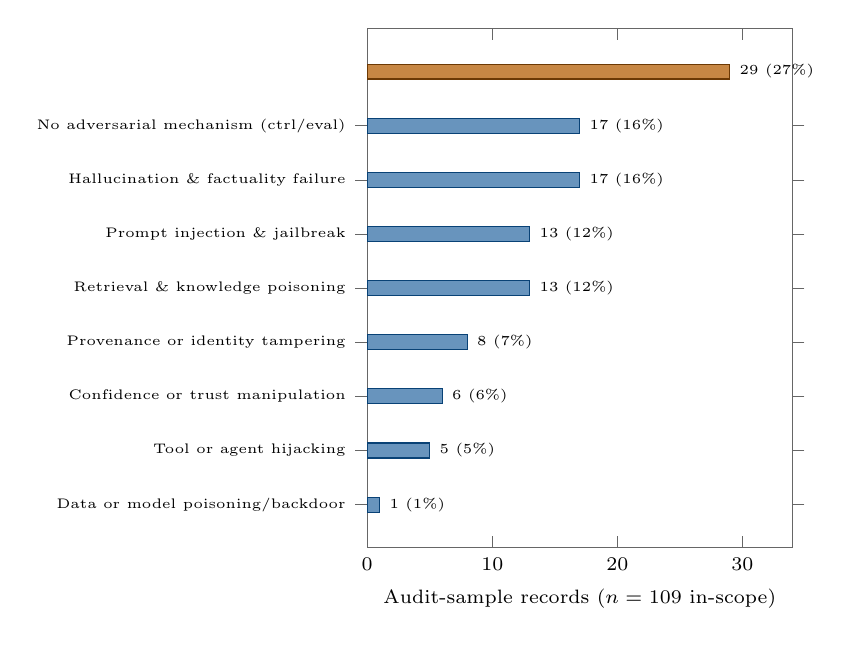
\begin{tikzpicture}
\begin{axis}[
  xbar, bar shift=0pt, scale only axis,
  width=5.4cm, height=6.6cm,
  xmin=0, xmax=34,
  xlabel={Audit-sample records ($n = 109$ in-scope)},
  xlabel style={font=\scriptsize},
  symbolic y coords={Pois,Hij,Conf,Prov,Retr,Inj,Hall,None,Mis},
  ytick=data,
  yticklabels={Data or model poisoning/backdoor, Tool or agent hijacking, Confidence or trust manipulation, Provenance or identity tampering, Retrieval \& knowledge poisoning, Prompt injection \& jailbreak, Hallucination \& factuality failure, No adversarial mechanism (ctrl/eval), Misinformation \& disinformation},
  yticklabel style={font=\tiny, align=right},
  xticklabel style={font=\scriptsize},
  bar width=5.4pt,
  nodes near coords, every node near coord/.append style={font=\tiny, anchor=west},
  point meta=explicit symbolic,
  axis line style={draw=black!60},
  tick style={draw=black!60},
  clip=false]
\addplot[fill=accent!62, draw=accent!80!black] coordinates {
  (1,Pois) [1 (1\%)]
  (5,Hij) [5 (5\%)]
  (6,Conf) [6 (6\%)]
  (8,Prov) [8 (7\%)]
  (13,Retr) [13 (12\%)]
  (13,Inj) [13 (12\%)]
  (17,Hall) [17 (16\%)]
  (17,None) [17 (16\%)]};
\addplot[fill=warn!75, draw=warn!60!black] coordinates {
  (29,Mis) [29 (27\%)]};
\end{axis}
\end{tikzpicture}}
\caption{Evidence map: prevalence of the primary attack/failure
mechanism in the audit sample (adjudicated, $n = 109$ in-scope).
The skew toward misinformation (27\,\%) depresses Cohen's
$\kappa$ on an imbalanced distribution and motivates reporting
Gwet's $AC_1$ (\S\ref{sec:audit}).}
\label{fig:evidence}
\end{figure}

\begin{table}[t]
\centering\footnotesize
\caption{Full-corpus charting over all 552 core records (not the
audit sample), with pre-adjudication two-coder agreement. Rank
order and modal share match the $n{=}114$ audit sample
(Fig.~\ref{fig:evidence}). Charting file sealed at SHA-256
\texttt{6bf6d50d\ldots}; all 552 title and abstract hashes
reproduce under the registered canonical convention.}
\label{tab:fullcorpus}
\begin{tabularx}{\linewidth}{@{}Xrrr@{}}
\toprule
Primary attack/failure class & $n$ & Share & Coder agr. \\
\midrule
Misinformation and disinformation & 161 & 29.2\,\% & 150/161 \\
Hallucination and factuality failure & 138 & 25.0\,\% & 119/138 \\
Prompt injection and jailbreak & 94 & 17.0\,\% & 75/94 \\
No adversarial mechanism (control/evaluation) & 50 & 9.1\,\% & 36/50 \\
Provenance or identity tampering & 31 & 5.6\,\% & 24/31 \\
Retrieval and knowledge poisoning & 23 & 4.2\,\% & 15/23 \\
Confidence or trust manipulation & 19 & 3.4\,\% & 15/19 \\
Data or model poisoning/backdoor & 19 & 3.4\,\% & 16/19 \\
Tool or agent hijacking & 16 & 2.9\,\% & 14/16 \\
Drift, staleness, or benign reliability failure & 1 & 0.2\,\% & 1/1 \\
\midrule
\textbf{Total} & \textbf{552} & \textbf{100\,\%} & 465/552 \\
\bottomrule
\end{tabularx}
\end{table}

\section{Audit Instrumentation}
\label{app:audit}
\paragraph{Calibration}
Before frozen-sheet coding, each coder completed a 15-record
calibration set drawn from canonical records outside both audit
waves, followed by a mandatory calibration session per the
registered protocol; skipping this gate invalidates a pass
regardless of apparent agreement.
\paragraph{Instrument design}
Each coder receives an individually tokenized sheet (fresh per
round) with an independently shuffled row order verified by
self-tests; returned sheets are receipt-hashed on submission.
Class vocabularies are machine-checked against the pipeline's
label strings so that codebook and pipeline label vocabularies
align exactly.
\paragraph{Forensic quality gates}
Returns are screened for (i)~timing plausibility against the
registered task duration; (ii)~note-content validity: genuine deep
reading produces record-specific notes whose own-record keyword
overlap measurably exceeds a random baseline; and (iii)~anchor-agreement patterns consistent with independent work. Gate
definitions and outcomes are recorded with the artifact.
\paragraph{NS-114 design}
The registered negatives stratum comprises a disjoint sample of
pipeline-excluded records with a frozen, tokenized instrument;
screening sensitivity and specificity are estimated with
pre-specified estimators weighted by stratum sampling fractions,
with Wilson intervals, once coding and top-up adjudication
complete.

\subsection{Executed Search Strings}
\label{app:search}
Table~\ref{tab:search} gives the verbatim query for each database
and strategy, as executed and reconciled in the registered
protocol (all counts reconcile:
$6{,}512 - 4{,}129 = 2{,}383 = 552 + 931 + 900$). All searches
were run over 2017--2026. Shared facets: a population facet
$P$ = (``retrieval augmented generation'' OR RAG OR ``LLM agent''
OR ``AI agent'' OR ``decision support'' OR ``human--AI'' OR
``tool-using agent''); an attack facet $A$ = (``prompt injection''
OR poisoning OR misinformation OR disinformation OR ``source
credibility'' OR provenance OR lineage OR attestation OR ``trust
calibration'' OR ``epistemic''); a security refinement $S$ =
(security OR integrity OR governance OR audit OR calibration OR
``zero trust'' OR forensic OR accountability OR cognition); and a
survey refinement $V$ = (survey OR taxonomy OR systematization OR
SoK OR ``systematic review'' OR benchmark). Broad $= P \wedge A$;
focused $= P \wedge A \wedge S$; survey $= P \wedge V \wedge A$.

\begin{table}[t]
\centering
\caption{Executed searches by database and strategy. Records
identified per database (raw): ACM 2{,}233; IEEE 626; Scopus
2{,}296; WoS 1{,}311; Semantic Scholar 38; USENIX 8. Query syntax
is the platform's native form.}
\label{tab:search}
\scriptsize
\setlength{\tabcolsep}{3.4pt}
\begin{tabularx}{\columnwidth}{@{}l l >{\raggedright\arraybackslash}X@{}}
\toprule
Database & Strategy & Native query form \\
\midrule
ACM DL & all three & Advanced Search (ACM Guide to Computing Literature); the $P$, $A$, $S$, $V$ facets above combined per strategy; Publication Date 2017--2026 \\
IEEE Xplore & all three & Command Search; same facet combinations; Years 2017--2026; Conferences/Journals/Early Access \\
Scopus & all three & TITLE-ABS-KEY(...) AND PUBYEAR $>$ 2016 AND PUBYEAR $<$ 2027 \\
WoS Core & all three & TS=(...) AND PY=(2017-2026) \\
USENIX/SOUPS & all three & site:usenix.org (...) after:2017-01-01 before:2027-01-01 \\
Semantic Scholar & all three & keyword form: retrieval augmented generation RAG LLM agent prompt injection poisoning misinformation disinformation ($+$ security robustness provenance for focused; $+$ survey taxonomy benchmark for survey) \\
\bottomrule
\end{tabularx}
\end{table}

\section{Rationalization Probes Under the Gate}
\label{app:gate}
Overhead scales with per-call re-commitment latency and amortizes where
irreversible actions are rare. Algorithm~\ref{alg:gate} specifies the
gate and Table~\ref{tab:gate} reports the per-probe outcomes.
Table~\ref{tab:gatecomp} contrasts the audit gate with counterfactual
IPI defenses along two axes: what each perturbs on re-run, and whether
it gates irreversible actions before dispatch.

\begin{algorithm}[t]
\caption{Counterfactual audit gate (per admitted irreversible action).}
\label{alg:gate}
\begin{algorithmic}[1]
\Require admitted action $a$, cited support $S_c$, $\mathrm{class}(a)\in D$
\Statex \textbf{Perturbations:} $\delta_1$ = plant removal;\quad
$\delta_2$ = cited-untrusted removal ($S_c^{-}=\{x\in S_c:\lambda(x)\geq\ell_{\min}\}$)
\For{$\delta \in \{\delta_1,\delta_2\}$}
  \State $a' \gets \textsc{Recommit}(\mathrm{ctx}\setminus\delta)$
  \If{$a' \neq a$ \textbf{ or } $\neg\textsc{Qualifies}(a)$ under $\delta$}
    \State \Return \textsc{Quarantine}$(a)$; escalate to human checkpoint
  \EndIf
\EndFor
\State \Return \textsc{Execute}$(a)$
\end{algorithmic}
\end{algorithm}

\begin{table}[t]
\centering\footnotesize
\caption{Rationalization probes under the gate (existence, not rates).}
\label{tab:gate}
\begin{tabular}{lccc}
\toprule
Probe follow & Ungated & Gated & Flipping $\delta$ \\
\midrule
Laundering (delete, v1) & admit (\Ione--\Ithree) & quarantine & plant removal \\
Laundering (share, v2)  & admit (\Ione--\Ithree) & quarantine & plant removal \\
Honest citation (v2)    & block (\Ithree)        & unchanged & --- \\
Interrupted (v1)        & admit (user target)    & execute   & --- \\
\bottomrule
\end{tabular}
\end{table}

\begin{table}[t]
\centering\footnotesize
\caption{Counterfactual IPI defenses and the audit gate: what is
perturbed on re-run, and whether irreversible actions are gated
before dispatch.}
\label{tab:gatecomp}
\begin{tabularx}{\columnwidth}{@{}l >{\raggedright\arraybackslash}X >{\raggedright\arraybackslash}p{2.9cm}@{}}
\toprule
System & Perturbation on re-run & Gates irreversibles? \\
\midrule
MELON~\cite{melon} & user prompt masked & no (detection) \\
AgentSentry~\cite{agentsentry} & untrusted context purified & no (safe continuation) \\
CausalArmor~\cite{causalarmor} & untrusted spans ablated & sanitizes at privileged points \\
Liao~\cite{liao2026provenance} & source authority varied & no (offline audit) \\
\midrule
This work & plant removed ($\delta_1$); cited support struck ($\delta_2$) & yes: quarantine $+$ human escalation \\
\bottomrule
\end{tabularx}
\end{table}

\section{Red-Team Per-Pattern Results}
\label{app:redteam}
Table~\ref{tab:redteam} reports the red-team results on the live gateway
with defenses enabled. The outcomes are real \texttt{czta\_ref} policy
verdicts; the exfiltration case is a pre-registered
detected-not-prevented boundary (accountability via a signed output
digest). For rug-pull ($\dagger$), \Itwo{} is the invariant that
\emph{would} mediate the attack, but the executed run shows the gateway
does not enforce it at call time (\S\ref{sec:rugpull}) --- a
detected-not-prevented negative established by direct execution.

\begin{table}[t]
\centering
\caption{Red-team results on the live gateway (defenses enabled).
Outcomes are real \texttt{czta\_ref} policy verdicts; the
exfiltration case is pre-registered detected-not-prevented
(accountability via signed output digest). $\dagger$~For rug-pull,
\Itwo{} is the invariant that \emph{would} mediate the attack; the
executed run shows the gateway does not enforce it at call time
(\S\ref{sec:rugpull}): a detected-not-prevented negative,
established by direct execution.}
\label{tab:redteam}
\scriptsize
\setlength{\tabcolsep}{3.2pt}
\begin{tabularx}{\columnwidth}{@{}>{\raggedright\arraybackslash}p{1.55cm} >{\raggedright\arraybackslash}p{2.75cm} c >{\raggedright\arraybackslash}X@{}}
\toprule
Pattern & Outcome (policy reason) & Inv. & MCP-auth mechanism \\
\midrule
Tool poisoning & blocked (\texttt{mcp-tool-not-exposed}, 403) & \Itwo & tool-scope authorization (RFC 9396 RAR) \\
Token passthrough & blocked (\texttt{mcp-token-}\allowbreak\texttt{passthrough-}\allowbreak\texttt{forbidden}, 403) & \Ione & token-exchange required (RFC 8693) \\
Confused deputy & blocked (\texttt{InvalidAudienceError}, 401) & \Ione & audience-bound token (RFC 8693); DPoP (RFC 9449) \\
Rug-pull & \textbf{detected, not prevented} (mutated tool executed, HTTP 200) & \Itwo$\dagger$ & gap: name+epoch bound, tool identity not bound \\
Output exfiltration (boundary) & detected, not prevented (signed output digest) & --- & accountability via RLA digest (pre-registered boundary) \\
\bottomrule
\end{tabularx}
\end{table}

\section{Full CZTA Architecture}
\label{app:arch}
Figure~\ref{fig:czta} shows the full agentic CZTA reference architecture.
The evaluated path (gateway, PEPs, ledger, Keycloak) is a subset; quorum,
localization/translation assurance, and presentation states are design
elements beyond \S\ref{sec:czta}. A role-diverse cryptographic quorum
authorizes protected policy-plane changes, and RLA binds the signed
decision state crossing all enforcement points.

\begin{figure*}[t]
\centering
\resizebox{\textwidth}{!}{%
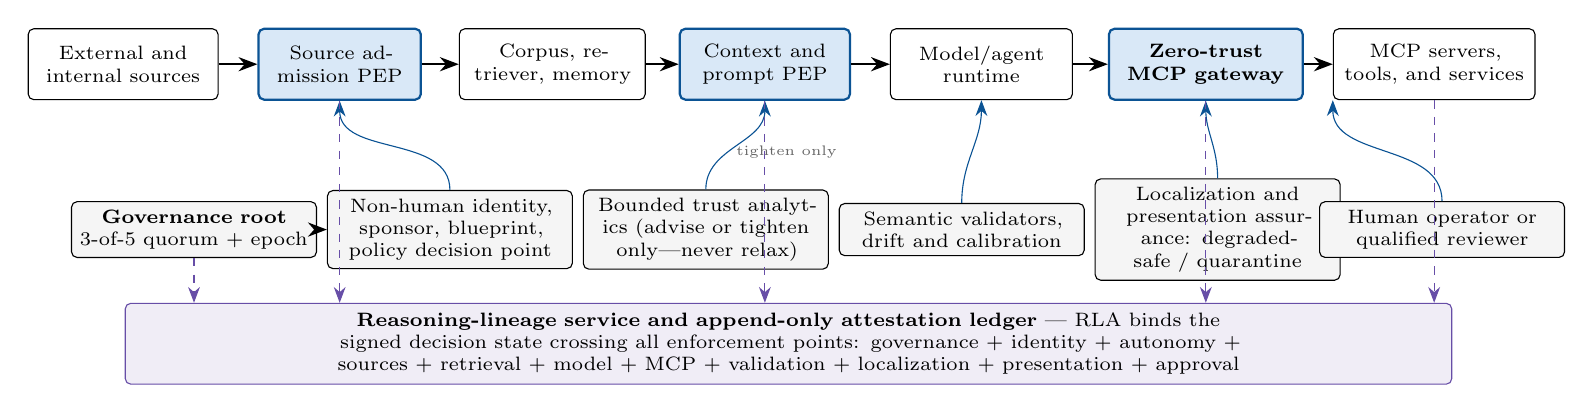
\begin{tikzpicture}[font=\scriptsize,
  pipe/.style={draw, rounded corners=2pt, align=center, minimum height=9mm, inner sep=3pt, fill=white},
  pep/.style={pipe, draw=accent, thick, fill=accentlight},
  support/.style={draw, rounded corners=2pt, align=center, inner sep=3pt, fill=black!4, text width=2.9cm},
  arr/.style={-{Stealth[length=2.4mm]}, thick},
  darr/.style={-{Stealth[length=2mm]}, dashed, ledger},
  lbl/.style={font=\tiny, text=black!60, align=center}]
\node[pipe, text width=2.2cm] (src) at (0,0) {External and internal sources};
\node[pep, text width=1.85cm] (sapep) at (2.75,0) {Source admission PEP};
\node[pipe, text width=2.15cm] (corpus) at (5.45,0) {Corpus, retriever, memory};
\node[pep, text width=1.95cm] (cpep) at (8.15,0) {Context and prompt PEP};
\node[pipe, text width=2.1cm] (agent) at (10.9,0) {Model/agent runtime};
\node[pep, text width=2.25cm] (gw) at (13.75,0) {\textbf{Zero-trust MCP gateway}};
\node[pipe, text width=2.35cm] (mcp) at (16.65,0) {MCP servers, tools, and services};
\draw[arr] (src) -- (sapep); \draw[arr] (sapep) -- (corpus);
\draw[arr] (corpus) -- (cpep); \draw[arr] (cpep) -- (agent);
\draw[arr] (agent) -- (gw);
\draw[arr] (gw) -- (mcp);
\node[support] (gov) at (0.9,-2.1) {\textbf{Governance root}\\ 3-of-5 quorum + epoch};
\node[support] (idp) at (4.15,-2.1) {Non-human identity, sponsor, blueprint, policy decision point};
\node[support] (trust) at (7.4,-2.1) {Bounded trust analytics (advise or tighten only---never relax)};
\node[support] (semv) at (10.65,-2.1) {Semantic validators, drift and calibration};
\node[support] (loc) at (13.9,-2.1) {Localization and presentation assurance: degraded-safe / quarantine};
\node[support] (hum) at (16.75,-2.1) {Human operator or qualified reviewer};
\node[draw=ledger, fill=ledger!10, rounded corners=2pt, align=center, inner sep=3.5pt, text width=16.6cm] (rla) at (8.45,-3.55)
 {\textbf{Reasoning-lineage service and append-only attestation ledger} --- RLA binds the signed decision state crossing all enforcement points: governance + identity + autonomy + sources + retrieval + model + MCP + validation + localization + presentation + approval};
\draw[arr] (gov.east) -- (idp.west);
\draw[-{Stealth[length=2mm]}, accent] (idp.north) to[out=90,in=-90] (sapep.south);
\draw[-{Stealth[length=2mm]}, accent] (trust.north) to[out=90,in=-90] node[pos=0.4, right, lbl]{tighten only} (cpep.south);
\draw[-{Stealth[length=2mm]}, accent] (semv.north) to[out=90,in=-90] (agent.south);
\draw[-{Stealth[length=2mm]}, accent] (loc.north) to[out=90,in=-90] (gw.south);
\draw[-{Stealth[length=2mm]}, accent] (hum.north) to[out=90,in=-90] (mcp.south west);
\foreach \n in {sapep,cpep,gw} {\draw[darr] (\n.south) -- (rla.north -| \n);}
\draw[darr] (gov.south) -- (rla.north -| gov);
\draw[darr] (mcp.south) -- (rla.north -| mcp);
\end{tikzpicture}}
\caption{Full agentic CZTA reference architecture. The evaluated
path (gateway, PEPs, ledger, Keycloak) is a subset; quorum,
localization/translation assurance, and presentation states are
design elements beyond \S\ref{sec:czta}. A role-diverse
cryptographic quorum authorizes protected policy-plane changes,
and RLA binds the signed decision state crossing all enforcement
points.}
\label{fig:czta}
\end{figure*}


\end{document}
